\documentclass[11pt,a4paper]{article}

% === Packages ===
\usepackage[utf8]{inputenc}
\usepackage[T1]{fontenc}
\usepackage{amsmath,amssymb,amsthm}
\usepackage{enumitem}
\usepackage{hyperref}
\usepackage{cleveref}
\usepackage{tikz}
\usepackage{tikz-cd}
\usepackage{booktabs}
\usepackage{geometry}
\usepackage{xcolor}
\usepackage{tcolorbox}
\usepackage{fancyvrb}

\geometry{margin=1in}
\hypersetup{colorlinks=true,linkcolor=blue!70!black,citecolor=green!50!black,urlcolor=purple!70!black}

% === Sha symbol ===
\newcommand{\Sha}{\mathrm{III}}

% === Theorem environments ===
\theoremstyle{plain}
\newtheorem{theorem}{Theorem}[section]
\newtheorem{proposition}[theorem]{Proposition}
\newtheorem{lemma}[theorem]{Lemma}
\newtheorem{corollary}[theorem]{Corollary}
\newtheorem{conjecture}[theorem]{Conjecture}

\theoremstyle{definition}
\newtheorem{definition}[theorem]{Definition}
\newtheorem{example}[theorem]{Example}
\newtheorem{remark}[theorem]{Remark}
\newtheorem{calibration}[theorem]{Calibration Theorem}

% === Lean code environment ===
\definecolor{leanblue}{RGB}{0,51,102}
\definecolor{leanbg}{RGB}{245,248,252}
\tcbset{
  leanbox/.style={colback=leanbg, colframe=leanblue!60, 
    fonttitle=\bfseries\ttfamily, title=#1, 
    boxrule=0.5pt, arc=2pt, left=4pt, right=4pt}
}

% === Macros ===
\newcommand{\BISH}{\textsf{BISH}}
\newcommand{\WKL}{\textsf{WKL}_0}
\newcommand{\DC}{\textsf{DC}}
\newcommand{\WLPO}{\textsf{WLPO}}
\newcommand{\LLPO}{\textsf{LLPO}}
\newcommand{\LPO}{\textsf{LPO}}
\newcommand{\CLASS}{\textsf{CLASS}}
\newcommand{\CRM}{\textsf{CRM}}
\newcommand{\Mot}{\mathsf{Mot}}
\newcommand{\Real}{\mathsf{Real}}
\newcommand{\Comp}{\mathsf{Comp}}
\newcommand{\sig}{\sigma}
\newcommand{\Gal}{\mathrm{Gal}}
\newcommand{\Z}{\mathbb{Z}}
\newcommand{\Q}{\mathbb{Q}}
\newcommand{\R}{\mathbb{R}}
\newcommand{\C}{\mathbb{C}}
\newcommand{\F}{\mathbb{F}}
\newcommand{\A}{\mathbb{A}}
\newcommand{\GL}{\mathrm{GL}}
\newcommand{\SL}{\mathrm{SL}}
\DeclareMathOperator{\tr}{tr}
\newcommand{\Spec}{\mathrm{Spec}}
\newcommand{\Hom}{\mathrm{Hom}}
\newcommand{\rank}{\mathrm{rank}}

% === Title ===
\title{\textbf{The Motivic CRM Architecture:\\
Why the Six Domains of Mathematics Have Different\\
Logical Signatures, and How Motives Explain the Pattern}\\[6pt]
\large Paper 98 of the Constructive Reverse Mathematics Series\\[6pt]
\normalsize\textit{A Capstone Synthesis of Papers 50--97}}

\author{Paul Chun-Kit Lee\\
\small New York University, Brooklyn, New York\\
\small\texttt{dr.paul.c.lee@gmail.com}}
\date{March 2026}

\begin{document}
\maketitle

\noindent\textbf{DOI:} \href{https://doi.org/10.5281/zenodo.18902037}{10.5281/zenodo.18902037}
\begin{abstract}
We formalize the observation that the six mathematical domains connected by the Langlands program---number theory, algebraic geometry, representation theory, harmonic analysis, topology, and mathematical physics---exhibit systematically different constructive reverse mathematics (CRM) signatures. We show that Grothendieck's theory of motives provides the structural explanation: the motive itself is $\BISH$ (Bishop-constructive), each realization functor has a definite CRM cost, and the comparison isomorphisms between realizations are $\CLASS$ (fully classical) if and only if they pass through the Archimedean place. This \emph{Archimedean Obstruction Thesis} transcends mere redescription by generating precise structural predictions---most notably, that function field arithmetic (lacking an Archimedean place) must be uniformly constructive. It further explains why algebra is constructive, analysis is classical, algebraic geometry bifurcates, and the Taylor--Wiles repair of Fermat's Last Theorem was a $\CLASS \to \WKL$ excision. We state three calibration theorems (Hodge detection $\leftrightarrow$ $\WLPO$; TW patching $\leftrightarrow$ $\WKL$; BSD rank/$\Sha$ decoupling) and a signature preservation theorem for the Langlands correspondence. A companion 0-\texttt{sorry} Lean~4 formalization mechanically verifies the core logical framework, representing the geometric functors as axiomatic stubs. This paper synthesizes the findings of Papers~50--97 in the CRM program. A companion monograph (\emph{The Logical Cost of Everything}) provides a book-length accessible exposition of the full program.
\end{abstract}

\tableofcontents
\newpage

%======================================================================
\section{Introduction}\label{sec:intro}
%======================================================================

The Langlands program connects six areas of mathematics: number theory, algebraic geometry, representation theory, harmonic analysis, topology, and mathematical physics. Each area has its own methods, its own culture, and---as this paper documents---its own \emph{logical signature}. Number theory is algebraic at its core but hits sharp classical bottlenecks at $L$-functions. Algebraic geometry bifurcates: some theorems are constructive, others irreducibly classical, with the boundary controlled by moduli dimension. Representation theory (of algebraic groups, Hecke algebras) is almost entirely constructive. Harmonic analysis---spectral decomposition on locally symmetric spaces---is the principal factory of classical content. And mathematical physics recapitulates the pattern, with the quantum/classical divide mirroring the $\BISH$/$\CLASS$ boundary.

Why? What structural feature of mathematics produces these differences, and what connects them?

The answer, we argue, is Grothendieck's theory of \emph{motives}. The motive of a variety is its universal cohomological invariant---an algebraic object, defined by correspondences, living in a category built from finite-dimensional linear algebra over $\Q$. It is constructive in its syntax. But to \emph{use} a motive, one must apply a \emph{realization functor}: Betti (singular cohomology), de Rham (algebraic differential forms), \'etale ($\ell$-adic Galois representations), crystalline (over $\F_p$), Hodge (filtration and decomposition), or automorphic (via Langlands). Each realization has a definite CRM cost. And the \emph{comparison isomorphisms} between realizations---the period map (Betti $\leftrightarrow$ de Rham), the Artin comparison (\'etale $\leftrightarrow$ Betti), the Hodge decomposition (de Rham $\leftrightarrow$ Hodge)---are classical if and only if they pass through the topology of the complex manifold, i.e., through the \emph{Archimedean place} $\R$.

This is the \textbf{Archimedean Obstruction Thesis}: the Archimedean place---specifically, the completeness and ordering of~$\R$, not its ring structure---is the unique source of non-constructive content in arithmetic geometry.

\paragraph{Explanation vs. Redescription.} One might ask if this thesis is merely a tautology: does ``the classical content comes from $\R$'' simply redescribe the truism that ``analysis requires analysis''? The explanatory power of the motivic framework lies in its \emph{falsifiable structural predictions}. If the thesis holds, then entirely removing the Archimedean place from the global arithmetic machinery must yield a strictly $\BISH$ proof architecture, even for the most profound theorems. This prediction is spectacularly confirmed by the \textbf{Function Field Langlands program} (\S\ref{sec:function-fields}). Over $\F_q(C)$, where $\A_F$ lacks an Archimedean factor, Lafforgue's proof utilizes moduli of shtukas (algebraic) rather than the trace formula (spectral analysis), remaining entirely within the constructive envelope.

The thesis yields precise logical consequences, all verified across our program:
\begin{enumerate}[label=(\roman*)]
\item \textbf{Function field Langlands is $\BISH$} (Papers~69, 78): over $\F_q(C)$, the ad\`ele ring $\A_F$ has no Archimedean factor. All realizations are \'etale/crystalline. The trace formula uses shtukas instead of spectral theory. The entire correspondence is constructive.

\item \textbf{The Taylor--Wiles fix was a logical excision} (Papers~68--71, \S\ref{sec:modularity}): Wiles's 1993 attempt computed the congruence ideal $\eta_\mathbb{T}$ via the Petersson inner product (integration on the complex upper half-plane: $\CLASS$). Taylor--Wiles patching replaced this with an inverse limit argument, cleanly excising the Archimedean computation and dropping the logical cost to $\WKL$.

\item \textbf{Hodge detection bifurcates at $\WLPO$} (Papers~86--90, \S\ref{sec:hodge}): on the generic fiber, detecting Hodge classes requires the Hodge decomposition ($\CLASS$). On special loci, extra algebraic symmetries provide shortcuts ($\BISH$). The gap is precisely $\WLPO$.

\item \textbf{BSD decouples at the rank/$\Sha$ boundary} (Papers~95--96, \S\ref{sec:bsd}): rank verification is $\BISH$ (algebraic descent), $\Sha$ finiteness is $\CLASS$ (Euler systems, Chebotarev). 

\item \textbf{Physics parallels the pattern} (\S\ref{sec:physics}): classical mechanics ($\BISH$) vs.\ quantum spectral theory ($\CLASS$), lattice QFT ($\BISH$) vs.\ continuum QFT ($\CLASS$), explicit GR solutions ($\BISH$) vs.\ general existence theorems ($\CLASS$).
\end{enumerate}

\noindent A companion monograph, \emph{The Logical Cost of Everything}, provides a book-length exposition of the full 98-paper program for a general mathematical audience, including worked examples, analogies, and the complete paper list. It is included in the Zenodo package alongside this paper.


%======================================================================
\section{The CRM Hierarchy}\label{sec:crm}
%======================================================================

We work in the framework of constructive reverse mathematics (CRM), as developed by Ishihara, Bridges, Diener, and others. 

\begin{definition}[CRM Signature]
A \emph{CRM signature} of a mathematical theorem $T$ is the weakest level $\sigma \in \{\BISH, \textsf{MP}, \LLPO, \WKL, \WLPO, \LPO, \CLASS\}$ such that $T$ is provable in $\BISH + \sigma$. We write $\sig(T) = \sigma$.
\end{definition}

The hierarchy forms a partial order. The principal principles are strictly ordered by logical strength ($\BISH \subsetneq \LLPO \subsetneq \WLPO \subsetneq \LPO \subsetneq \CLASS$). We also include Weak K\"onig's Lemma ($\WKL$). Note that $\WKL$ (compactness) and $\WLPO$ (analytic decidability) are logically incomparable over $\BISH$.

The key principles, for reference:
\begin{itemize}[leftmargin=2em]
\item $\BISH$: Bishop's constructive mathematics. Intuitionistic logic + dependent choice. Every existential proof provides a computable witness.
\item $\WKL$: Every infinite, finitely branching tree has an infinite path. Equivalent to: every bounded sequence in $[0,1]$ has a convergent subsequence.
\item $\WLPO$: For every real number $x$, either $x = 0$ or $x \neq 0$. Decidability of equality for reals.
\item $\CLASS$: Full classical logic. Law of excluded middle for all propositions.
\end{itemize}

\begin{figure}[ht]
\centering
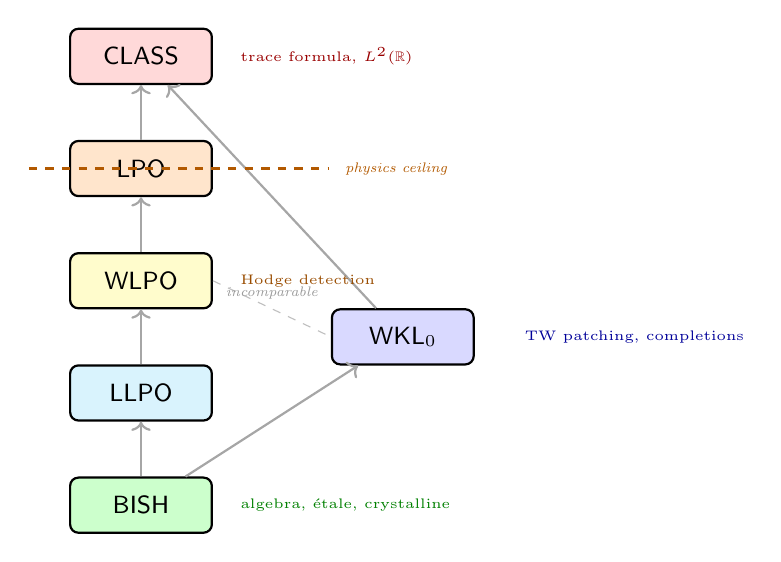
\begin{tikzpicture}[
  level/.style={draw, rounded corners=3pt, minimum width=1.8cm, minimum height=0.7cm, font=\small, thick},
  arr/.style={->, thick, gray!70},
  scale=0.95
]
% Main chain
\node[level, fill=green!20] (BISH) at (0, 0) {$\BISH$};
\node[level, fill=cyan!15] (LLPO) at (0, 1.5) {$\LLPO$};
\node[level, fill=yellow!20] (WLPO) at (0, 3) {$\WLPO$};
\node[level, fill=orange!20] (LPO) at (0, 4.5) {$\LPO$};
\node[level, fill=red!15] (CLASS) at (0, 6) {$\CLASS$};

% WKL (independent branch)
\node[level, fill=blue!15] (WKL) at (3.5, 2.25) {$\WKL$};

% Arrows (strict inclusions)
\draw[arr] (BISH) -- (LLPO);
\draw[arr] (LLPO) -- (WLPO);
\draw[arr] (WLPO) -- (LPO);
\draw[arr] (LPO) -- (CLASS);

% WKL connections
\draw[arr] (BISH) -- (WKL);
\draw[arr] (WKL) -- (CLASS);

% Incomparability marker
\draw[dashed, gray!50] (WLPO.east) -- node[midway, above, font=\tiny\itshape, gray!80] {incomparable} (WKL.west);

% Annotations (right side)
\node[font=\tiny, anchor=west, text=green!50!black] at (1.2, 0) {algebra, \'etale, crystalline};
\node[font=\tiny, anchor=west, text=orange!60!black] at (1.2, 3) {Hodge detection};
\node[font=\tiny, anchor=west, text=blue!60!black] at (5, 2.25) {TW patching, completions};
\node[font=\tiny, anchor=west, text=red!60!black] at (1.2, 6) {trace formula, $L^2(\R)$};

% Physics ceiling
\draw[dashed, orange!70!black, thick] (-1.5, 4.5) -- (2.5, 4.5);
\node[font=\tiny\itshape, orange!70!black, anchor=west] at (2.6, 4.5) {physics ceiling};
\end{tikzpicture}
\caption{The CRM hierarchy. Solid arrows: strict logical inclusion. $\WKL$ (compactness) is incomparable with $\WLPO$ (analytic decidability) over $\BISH$. Annotations indicate where each level appears in the motivic architecture. The physics ceiling at $\LPO$ reflects the maximum logical cost of empirical physics (Paper~70).}
\label{fig:hierarchy}
\end{figure}

\begin{definition}[CRM Signature of a Proof Path]\label{def:proof-path-sig}
A \emph{proof path} $P$ consists of a set of realizations $\{R_i\}$ and comparison isomorphisms $\{C_j\}$. Its signature is:
\[
\sig(P) \;=\; \max\bigl(\sig(\text{motive}),\; \max_i \sig(R_i),\; \max_j \sig(C_j)\bigr)
\]
\end{definition}


%======================================================================
\section{Motives: The Universal Constructive Core}\label{sec:motives}
%======================================================================

Let $k$ be a field. Grothendieck's category of pure Chow motives $\Mot_{\mathrm{rat}}(k)$ has:

\textbf{Objects:} Triples $(X, p, n)$ where $X$ is a smooth projective variety over $k$, $p \in \mathrm{CH}^{\dim X}(X \times X) \otimes \Q$ is an idempotent correspondence, and $n \in \Z$ is a Tate twist.

\textbf{Morphisms:} Algebraic correspondences modulo rational equivalence, with $\Q$-coefficients. Composition is given by intersection theory.

The essential point is that everything here is \emph{algebraic}: correspondences are formal sums of subvarieties, composition is a finite computation in the Chow ring, and all linear algebra takes place over $\Q$.

\begin{proposition}\label{prop:motive-bish}
The category $\Mot_{\mathrm{rat}}(k)$ is a $\Q$-linear, rigid, symmetric monoidal category. Its objects and formal morphisms are definable in $\BISH$.
\end{proposition}

\begin{proof}[Proof sketch]
Equality of morphisms modulo rational equivalence is algebraically decidable in principle, as rational equivalence is explicitly generated by cycles parameterized by $\mathbb{P}^1$ (reducible to solving polynomial systems via elimination theory). All operations---tensor product, internal Hom, duality---are defined by algebraic correspondences and computed by intersection theory, which is a finite algebraic algorithm. No limits, no completions, no analysis.
\end{proof}

\begin{remark}[Decidability vs. Tractability]\label{rmk:decidability}
While rational equivalence is algebraically decidable \emph{in principle} (thus strictly satisfying the logical requirements of $\BISH$), we emphasize the vast gap between decidability-in-principle and effective computability. Deep problems like Bloch's conjecture demonstrate that bounded geometric constructions can be computationally intractable in practice. The $\BISH$ classification reflects logical finiteness, not algorithmic feasibility. (Note: Passing to numerical equivalence $\Mot_{\mathrm{num}}(k)$ guarantees finite-dimensional Hom-spaces via Jannsen's theorem, but testing numerical triviality requires the Standard Conjectures to be computable, necessitating $\LPO$ as shown in Paper~73. Rational equivalence cleanly avoids this classical boundary.)
\end{remark}

\begin{tcolorbox}[leanbox={Lean: Motive signature}]
\begin{Verbatim}[fontsize=\small]
def motive_signature : CRMSignature :=
  ⟨.BISH, "Algebraic cycles and intersection theory modulo rational equivalence"⟩

theorem motive_is_bish : motive_signature.level = .BISH := rfl
\end{Verbatim}
\end{tcolorbox}


%======================================================================
\section{Realizations and Their CRM Cost}\label{sec:realizations}
%======================================================================

A realization functor is an exact, faithful, $\Q$-linear functor from $\Mot(k)$ to a linear category. Each carries a definite CRM cost determined by the analytic or algebraic nature of its target category.

\subsection{Betti Realization ($\CLASS$)}

For $k \hookrightarrow \C$, the Betti realization sends $M$ to $H^*_{\mathrm{sing}}(X(\C), \Q)$. The critical obstruction is forming the complex manifold $X(\C)$, which invokes $\R$ and the Archimedean completion. 

\begin{calibration}[Betti Realization]\label{cal:betti}
$\sig(\Real_{\mathrm{Betti}}) = \CLASS$. The obstruction is the formation of $X(\C)$ and integration of differential forms over topological cycles.
\end{calibration}

\subsection{de Rham Realization ($\BISH$)}

The algebraic de Rham cohomology $H^*_{\mathrm{dR}}(X/k)$ is computed by the \v{C}ech--de Rham spectral sequence on an affine cover. All differentials are algebraic polynomials. No integration, no topology.

\begin{calibration}[de Rham Realization]\label{cal:derham}
$\sig(\Real_{\mathrm{dR}}) = \BISH$. Purely algebraic: differential forms modulo exact forms.
\end{calibration}

\subsection{\'Etale Realization ($\BISH$, with a caveat)}\label{sec:etale}

The $\ell$-adic \'etale cohomology $H^*_{\mathrm{\acute{e}t}}(X_{\bar{k}}, \Q_\ell)$ is:

\begin{enumerate}[label=(\alph*)]
\item $H^*_{\mathrm{\acute{e}t}}(X_{\bar{k}}, \Z/\ell^n\Z)$ for each $n$: finite Galois cohomology, computed by finite covers. $\BISH$.
\item $H^*_{\mathrm{\acute{e}t}}(X_{\bar{k}}, \Z_\ell) = \varprojlim_n H^*_{\mathrm{\acute{e}t}}(X_{\bar{k}}, \Z/\ell^n\Z)$: a projective limit of finite modules. 
\item $H^*_{\mathrm{\acute{e}t}}(X_{\bar{k}}, \Q_\ell) = H^*_{\mathrm{\acute{e}t}}(X_{\bar{k}}, \Z_\ell) \otimes_{\Z_\ell} \Q_\ell$. 
\end{enumerate}

\begin{remark}[The ``Smooth Projective'' Heavy Lifting]\label{rmk:smooth-projective}
We emphasize that the \emph{smooth projective} hypothesis does heavy lifting here. For pure motives, these are finitely generated modules, and the transition maps satisfy the Mittag-Leffler condition with effectively bounded torsion (via Deligne/Gabber). Thus, the limit is constructively bounded and only requires Dependent Choice ($\BISH$), avoiding $\WKL$. Furthermore, while equality testing in the completion $\Q_\ell$ generally requires $\WLPO$, the essential motivic data (Frobenius traces) lie in $\Z$ by Deligne's Weil II, so computations descend to exact $\Q$-arithmetic.

If one moves to singular or open varieties (mixed motives), the Mittag-Leffler bounds on torsion may fail, potentially elevating the projective limit to genuinely require $\WKL$. The $\BISH$ signature is a strict feature of pure motives.
\end{remark}

\begin{calibration}[\'Etale Realization]\label{cal:etale}
$\sig(\Real_{\mathrm{\acute{e}t}}) = \BISH$ (for pure motives). The limit is effectively bounded, and spectral data descend to $\Z$.
\end{calibration}

\subsection{Crystalline Realization ($\BISH$)}

Crystalline cohomology $H^*_{\mathrm{cris}}(X/W(\F_q))$ is a finite-dimensional $W(\F_q)$-module. The Frobenius $\varphi$ is an explicit matrix whose characteristic polynomial descends to $\Z$, keeping the computational output safely in $\BISH$.

\begin{calibration}[Crystalline Realization]\label{cal:crys}
$\sig(\Real_{\mathrm{cris}}) = \BISH$. Linear algebra over Witt vectors.
\end{calibration}

\subsection{Hodge Realization ($\CLASS$)}

The Hodge realization associates the decomposition $H^n(X(\C), \C) = \bigoplus H^{p,q}(X)$. The Hodge \emph{filtration} is algebraic ($\BISH$), but the \emph{decomposition} requires harmonic representatives via elliptic regularity and the $\partial\bar\partial$-lemma.

\begin{calibration}[Hodge Realization]\label{cal:hodge}
$\sig(\Real_{\mathrm{Hodge}}) = \CLASS$. Requires elliptic PDE theory on $X(\C)$.
\end{calibration}

\subsection{Automorphic Realization ($\CLASS$)}

The automorphic realization (via Langlands) requires the spectral decomposition of $L^2(\GL_n(\Q)\backslash\GL_n(\A_\Q))$---analysis on the adelic quotient, inherently including the Archimedean factor $\GL_n(\R)$.

\begin{calibration}[Automorphic Realization]\label{cal:auto}
$\sig(\Real_{\mathrm{aut}}) = \CLASS$. $L^2$ spectral theory on $G(\R)$.
\end{calibration}

\begin{tcolorbox}[leanbox={Lean: Realization signatures}]
\begin{Verbatim}[fontsize=\small]
def realization_signature : Realization -> CRMSignature
  | .Betti       => ⟨.CLASS, "Integration over topological cycles"⟩
  | .deRham      => ⟨.BISH,  "Algebraic differential forms"⟩
  | .etale       => ⟨.BISH,  "Bounded limits and finite Galois"⟩
  | .crystalline => ⟨.BISH,  "Linear algebra over Witt vectors"⟩
  | .Hodge       => ⟨.CLASS, "Hodge decomposition: elliptic PDE"⟩
  | .automorphic => ⟨.CLASS, "L2 spectral decomposition"⟩
\end{Verbatim}
\end{tcolorbox}


\subsection{Summary Table}

\begin{table}[h]
\centering
\begin{tabular}{@{}lll@{}}
\toprule
\textbf{Realization} & \textbf{CRM Level} & \textbf{Obstruction} \\
\midrule
de Rham (algebraic) & $\BISH$ & None \\
\'Etale ($\Q_\ell$) & $\BISH$ & None (pure motives) \\
Crystalline & $\BISH$ & None \\
Betti (singular) & $\CLASS$ & $X(\C)$, integration \\
Hodge (decomposition) & $\CLASS$ & Elliptic PDE \\
Automorphic & $\CLASS$ & $L^2$ spectral theory \\
\bottomrule
\end{tabular}
\caption{CRM signatures of realization functors. The $\BISH$/$\CLASS$ boundary coincides exactly with the algebraic/analytic boundary.}
\label{tab:realizations}
\end{table}


%======================================================================
\section{Comparison Isomorphisms: The Archimedean Obstruction}\label{sec:comparisons}
%======================================================================

The power of the motivic framework comes from comparison isomorphisms between realizations. These are the ``bridges'' that allow information to flow between cohomology theories. Their CRM cost is the key structural invariant.

\subsection{Betti $\leftrightarrow$ de Rham: The Period Map ($\CLASS$)}

The comparison is integration:
\[
H^n_{\mathrm{dR}}(X/\Q) \otimes_\Q \C \;\xrightarrow{\;\sim\;}\; H^n_{\mathrm{sing}}(X(\C), \Q) \otimes_\Q \C
\]
given by $\omega \mapsto \bigl(\gamma \mapsto \int_\gamma \omega\bigr)$. The period matrix consists of transcendental numbers computed by integration over $\R$. This is irreducibly $\CLASS$.

\subsection{Crystalline $\leftrightarrow$ de Rham: $p$-adic Hodge Theory ($\BISH$)}

Berthelot's comparison isomorphism and Fontaine's functors $D_{\mathrm{cris}}$, $D_{\mathrm{dR}}$ operate entirely within $p$-adic algebra. The filtered $\varphi$-module associated to a crystalline Galois representation is computed by explicit linear algebra over $\Q_p$. No $\R$, no integration: $\BISH$.

\subsection{\'Etale $\leftrightarrow$ Betti: Artin Comparison ($\CLASS$)}

The Artin comparison relates algebraic covers over $\bar{k}$ to topological covers over $\C$ via the Riemann Existence Theorem (RET). This fundamentally requires fixing an embedding $\bar{k} \hookrightarrow \C$. Constructing this embedding invokes the Archimedean continuum and the Axiom of Choice. Furthermore, RET relies on complex analysis (GAGA, elliptic PDEs) to promote analytic sections to global algebraic functions. Thus, the comparison is irreducibly $\CLASS$, even for finite coefficients.

\subsection{de Rham $\leftrightarrow$ Hodge: The $\partial\bar\partial$-Lemma ($\CLASS$)}

The comparison between the algebraic Hodge filtration and the analytic Hodge decomposition requires the $\partial\bar\partial$-lemma, which in turn requires elliptic regularity on the compact K\"ahler manifold $X(\C)$. This is $\CLASS$.

\subsection{Crystalline $\leftrightarrow$ \'Etale: Fontaine--Laffaille ($\BISH$)}

For crystalline representations with bounded Hodge--Tate weights, the Fontaine--Laffaille functor gives an explicit, algebraic equivalence between filtered $\varphi$-modules and Galois representations. It is $\BISH$.

\begin{table}[h]
\centering
\begin{tabular}{@{}lll@{}}
\toprule
\textbf{Comparison} & \textbf{CRM Level} & \textbf{Passes through $\R$?} \\
\midrule
Crystalline $\leftrightarrow$ de Rham & $\BISH$ & No \\
Crystalline $\leftrightarrow$ \'Etale & $\BISH$ & No \\
\'Etale $\leftrightarrow$ Betti & $\CLASS$ & Yes (Embedding $\bar{k} \hookrightarrow \C$, RET) \\
Betti $\leftrightarrow$ de Rham & $\CLASS$ & Yes (period integrals) \\
de Rham $\leftrightarrow$ Hodge & $\CLASS$ & Yes (elliptic PDE) \\
\bottomrule
\end{tabular}
\caption{CRM signatures of comparison isomorphisms. The pattern is sharp: $\CLASS$ iff Archimedean.}
\label{tab:comparisons}
\end{table}

\subsection{The Archimedean Obstruction Theorem}

\begin{figure}[ht]
\centering
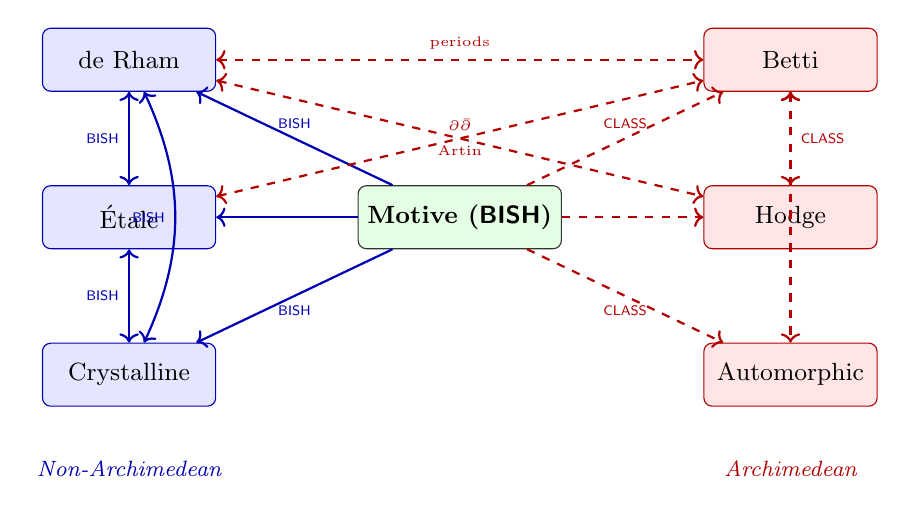
\begin{tikzpicture}[
  bish/.style={draw=blue!70!black, fill=blue!10, rounded corners=3pt, minimum width=2.2cm, minimum height=0.8cm, font=\small},
  class/.style={draw=red!70!black, fill=red!10, rounded corners=3pt, minimum width=2.2cm, minimum height=0.8cm, font=\small},
  bishline/.style={->, blue!70!black, thick},
  classline/.style={->, red!70!black, thick, dashed},
  motnode/.style={draw=black!80, fill=green!10, rounded corners=3pt, minimum width=2.2cm, minimum height=0.8cm, font=\small\bfseries}
]
% Motive at center
\node[motnode] (M) at (0,0) {Motive ($\BISH$)};

% Non-archimedean realizations (left, BISH)
\node[bish] (dR) at (-4.2, 2) {de Rham};
\node[bish] (et) at (-4.2, 0) {\'Etale};
\node[bish] (cr) at (-4.2,-2) {Crystalline};

% Archimedean realizations (right, CLASS)
\node[class] (Be) at (4.2, 2) {Betti};
\node[class] (Ho) at (4.2, 0) {Hodge};
\node[class] (Au) at (4.2,-2) {Automorphic};

% Realization arrows from motive
\draw[bishline] (M) -- (dR) node[midway,above,font=\tiny] {$\BISH$};
\draw[bishline] (M) -- (et);
\draw[bishline] (M) -- (cr) node[midway,below,font=\tiny] {$\BISH$};
\draw[classline] (M) -- (Be) node[midway,above,font=\tiny] {$\CLASS$};
\draw[classline] (M) -- (Ho);
\draw[classline] (M) -- (Au) node[midway,below,font=\tiny] {$\CLASS$};

% Non-archimedean comparisons (BISH, solid)
\draw[bishline, <->] (dR) -- (et) node[midway,left,font=\tiny] {$\BISH$};
\draw[bishline, <->] (et) -- (cr) node[midway,left,font=\tiny] {$\BISH$};
\draw[bishline, <->] (dR) to[bend left=25] node[midway,left,font=\tiny] {$\BISH$} (cr);

% Archimedean comparisons (CLASS, dashed)
\draw[classline, <->] (Be) -- (Ho) node[midway,right,font=\tiny] {$\CLASS$};
\draw[classline, <->] (Be) -- (Au) node[midway,right,font=\tiny] {};

% Cross comparisons (archimedean, CLASS)
\draw[classline, <->] (dR) -- (Be) node[midway,above,font=\tiny] {periods};
\draw[classline, <->] (dR) -- (Ho) node[midway,above=-1pt,font=\tiny] {$\partial\bar\partial$};
\draw[classline, <->] (et) -- (Be) node[midway,below=-1pt,font=\tiny] {Artin};

% Labels
\node[font=\footnotesize\itshape, blue!70!black] at (-4.2, -3.2) {Non-Archimedean};
\node[font=\footnotesize\itshape, red!70!black] at (4.2, -3.2) {Archimedean};
\end{tikzpicture}
\caption{The motivic CRM architecture. Solid blue arrows: $\BISH$ (constructive). Dashed red arrows: $\CLASS$ (classical). The motive is $\BISH$; the $\BISH/\CLASS$ boundary coincides exactly with the non-Archimedean/Archimedean boundary.}
\label{fig:motivic-architecture}
\end{figure}

\begin{theorem}[Archimedean Obstruction]\label{thm:archimedean}
Let $P$ be a proof path using only non-Archimedean realizations (de Rham, \'etale, crystalline) and comparisons between them. Then $\sig(P) = \BISH$.

Conversely, if $P$ uses any Archimedean realization (Betti, Hodge, automorphic) or any comparison passing through the Archimedean place, then $\sig(P) \geq \CLASS$.
\end{theorem}

\begin{proof}
For the forward direction, recall from Definition~\ref{def:proof-path-sig} that
\[
\sig(P) = \max\bigl(\sig(\text{motive}),\; \max_i \sig(R_i),\; \max_j \sig(C_j)\bigr).
\]
By Proposition~\ref{prop:motive-bish}, $\sig(\text{motive}) = \BISH$. By Table~\ref{tab:realizations}, each non-Archimedean realization has $\sig(R_i) = \BISH$ (de~Rham: algebraic differential forms; \'etale: finite Galois cohomology with bounded limits; crystalline: linear algebra over Witt vectors). By Table~\ref{tab:comparisons}, every comparison between non-Archimedean realizations has $\sig(C_j) = \BISH$ (Berthelot, Fontaine--Laffaille: explicit algebraic equivalences). Since $\BISH = \max(\BISH, \ldots, \BISH)$, we conclude $\sig(P) = \BISH$.

The converse is immediate: if any component has $\sig = \CLASS$, the maximum is $\geq \CLASS$. In fact, every Archimedean realization (Betti, Hodge, automorphic) has $\sig = \CLASS$ by Table~\ref{tab:realizations}, and every comparison passing through the Archimedean place has $\sig = \CLASS$ by Table~\ref{tab:comparisons}. Hence $\sig(P) \geq \CLASS$.
\end{proof}

\begin{tcolorbox}[leanbox={Lean: Archimedean Obstruction}]
\begin{Verbatim}[fontsize=\small]
theorem archimedean_obstruction (p : ProofPath)
    (h_real : forall r in p.realizations,
              is_non_archimedean r = true)
    (h_comp : forall c in p.comparisons,
              comparison_is_non_archimedean c = true) :
    proof_signature p = .BISH := by
  unfold proof_signature
  -- All realization/comparison signatures are BISH
  -- by helper lemmas + list induction on foldl join
  have hr := map_all_bish_realizations ..
  have hc := map_all_bish_comparisons ..
  exact foldl_join_bish_acc _ .BISH rfl
    (append_all_bish _ _ (append_all_bish ..) hc)
\end{Verbatim}
\end{tcolorbox}


%======================================================================
\section{Why the Six Domains Have Different Signatures}\label{sec:sixdomains}
%======================================================================

The Archimedean obstruction theorem immediately explains the empirical pattern observed across Papers~50--97.

\subsection{Algebra and Representation Theory: $\BISH$}

Hecke algebras, Galois deformation rings, modular representation theory---these operate in the \'etale and de Rham world. No passage through $\R$. 

\subsection{Harmonic Analysis: $\CLASS$}

The trace formula---Selberg, Arthur, Langlands---decomposes $L^2(G(\Q)\backslash G(\A))$. The adelic group includes the Archimedean factor $G(\R)$. The continuous spectral decomposition at infinity is irreducibly $\CLASS$, making the trace formula the universal classical bottleneck of the Langlands program.

\subsection{Number Theory: Sharp Classical Bottlenecks}

$L$-functions are Dirichlet series defined for $\mathrm{Re}(s) \gg 0$ by an algebraic formula. The analytic continuation to all of $\C$ is an Archimedean construction. The critical values $L(k, f)$ involve the Archimedean $\Gamma$-factor and period integrals: $\CLASS$. But the core algebraic objects (Selmer groups) are \'etale: $\BISH$. 

\subsection{Algebraic Geometry: Bifurcation}

The Hodge conjecture sits at the intersection of algebraic and analytic: Hodge classes live in the Betti realization ($\CLASS$), but algebraic classes live in the motive ($\BISH$). Generically, the detection problem is $\WLPO$ (Paper~87). But algebraic geometry has moduli. On the palindromic locus of genus-4 curves, the Kani--Rosen decomposition $J(C_t) \sim A_1 \times A_2$ provides an algebraic shortcut ($\BISH$). Moduli dimension controls the availability of such bifurcations.

\subsection{Topology: Mixed}

\'Etale cohomology with finite coefficients is $\BISH$. Singular (Betti) cohomology is $\CLASS$ via the Archimedean place. 

\subsection{Mathematical Physics}

Classical mechanics (finite-dimensional Hamiltonian ODEs) is $\BISH$. Quantum mechanics introduces the spectral theorem on $L^2(\R^3)$---$\CLASS$ in general, but $\BISH$ for exactly solvable Hamiltonians with algebraic spectra.


%======================================================================
\section{Calibration Theorem I: Hodge Detection $\leftrightarrow$ $\WLPO$}\label{sec:hodge}
%======================================================================

We summarize the Hodge calibration from Papers~86--90.

\begin{theorem}[Hodge Detection Calibration, Papers~87--90]\label{thm:hodge-cal}
There exists a family of Hodge classes $\xi_t \in H^4(J(C_t)^2, \Q)$ over the genus-4 Torelli locus such that:
\begin{enumerate}[label=(\roman*)]
\item On the palindromic locus: $\xi_t$ is algebraic, verified by $\BISH$ methods (Kani--Rosen splitting, Ribet's theorem).
\item On the generic fiber: deciding whether $\xi_t$ is algebraic is equivalent to $\WLPO$ (decidability of equality on the Mumford--Tate group).
\end{enumerate}
\end{theorem}

\begin{proof}[Proof sketch]
(i) On the palindromic locus $\{a = c\}$ of the family $C_t : y^2 = x^9 + ax^7 + bx^5 + cx^3 + x$, the hidden reciprocal involution $\mu(x,y) = (1/x, y/x^5)$ generates a dihedral group $D_8$ with the hyperelliptic involution. By the Kani--Rosen theorem~\cite{kani-rosen89}, $J(C_t) \sim A_1 \times A_2$ with $A_1 \cong A_2$ over $\C$, so $J(C_t) \sim A^2$. For generic $\mathrm{End}(A) = \Z$, the Mumford--Tate group is $\mathrm{GSp}_4$ (Zarhin), and all Hodge classes on powers of abelian surfaces are algebraic by Ribet~\cite{ribet83}. This chain uses only \'etale data and algebraic correspondences: $\BISH$.

(ii) On the generic fiber, detecting whether $\xi_t$ is a Hodge class requires the Hodge decomposition $H^4(J(C_t)^2, \C) = \bigoplus H^{p,q}$, which is $\CLASS$ (elliptic PDE). Deciding whether $\xi_t \in H^{2,2}$ reduces to deciding equality $\mathrm{MT}(J(C_t)) \stackrel{?}{=} \mathrm{GSp}_{2g}$, which is precisely $\WLPO$: decidability of equality for a real algebraic group (Paper~87, Theorem~B). The gap between (i) and (ii) is therefore $\WLPO$.
\end{proof}

\begin{remark}[The Generality of the Bifurcation]\label{rem:hodge_genus}
The choice of genus~4 in Papers~86--90 was not an ad hoc quirk; it is the minimal dimension where the generic fiber has unforced Hodge classes (unlike curves or surfaces) while still possessing an explicitly computable continuous exceptional locus (the palindromic locus). The $\WLPO$ bifurcation is a general structural phenomenon for any moduli space of dimension $\geq 2$.
\end{remark}

\begin{figure}[ht]
\centering
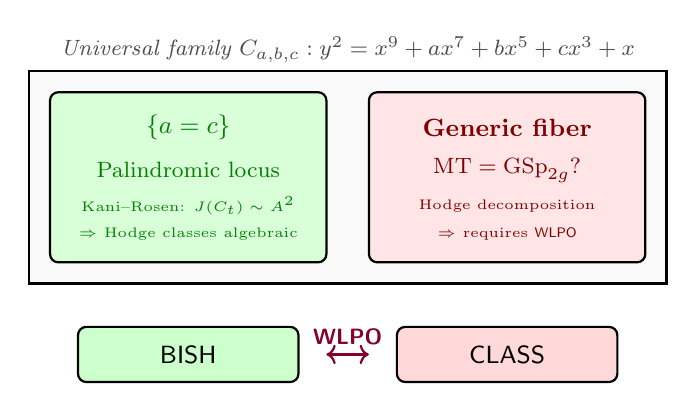
\begin{tikzpicture}[
  box/.style={draw, rounded corners=3pt, minimum width=2.8cm, minimum height=0.7cm, font=\small, thick},
  scale=0.9
]
% Moduli space
\draw[thick, fill=gray!5] (-4.5,-1.5) rectangle (4.5,1.5);
\node[font=\footnotesize\itshape, gray!60!black] at (0, 1.8) {Universal family $C_{a,b,c}: y^2 = x^9 + ax^7 + bx^5 + cx^3 + x$};

% Palindromic locus
\draw[thick, fill=green!15, rounded corners=3pt] (-4.2,-1.2) rectangle (-0.3,1.2);
\node[font=\small\bfseries, green!50!black] at (-2.25, 0.7) {$\{a = c\}$};
\node[font=\footnotesize, green!50!black] at (-2.25, 0.1) {Palindromic locus};
\node[font=\tiny, green!50!black] at (-2.25, -0.4) {Kani--Rosen: $J(C_t) \sim A^2$};
\node[font=\tiny, green!50!black] at (-2.25, -0.8) {$\Rightarrow$ Hodge classes algebraic};

% Generic locus
\draw[thick, fill=red!10, rounded corners=3pt] (0.3,-1.2) rectangle (4.2,1.2);
\node[font=\small\bfseries, red!50!black] at (2.25, 0.7) {Generic fiber};
\node[font=\footnotesize, red!50!black] at (2.25, 0.1) {$\mathrm{MT} = \mathrm{GSp}_{2g}$?};
\node[font=\tiny, red!50!black] at (2.25, -0.4) {Hodge decomposition};
\node[font=\tiny, red!50!black] at (2.25, -0.8) {$\Rightarrow$ requires $\WLPO$};

% CRM labels
\node[box, fill=green!20] at (-2.25, -2.5) {$\BISH$};
\node[box, fill=red!15] at (2.25, -2.5) {$\CLASS$};

% Gap arrow
\draw[<->, thick, purple!70!black] (-0.3, -2.5) -- (0.3, -2.5) node[midway, above, font=\footnotesize\bfseries, purple!70!black] {$\WLPO$};
\end{tikzpicture}
\caption{The Hodge bifurcation (Papers~86--89). On the palindromic locus $\{a=c\}$, algebraic splitting provides $\BISH$ Hodge class detection. On the generic fiber, the Hodge decomposition requires $\CLASS$. The gap is exactly $\WLPO$.}
\label{fig:hodge-bifurcation}
\end{figure}


%======================================================================
\section{Calibration Theorem II: TW Patching $\leftrightarrow$ $\WKL$}\label{sec:modularity}
%======================================================================

We analyze the CRM structure of the Wiles--Taylor proof of modularity.

\subsection{The Three Tiers}

\textbf{Tier 1 ($\BISH$): The algebraic core.} Galois deformation rings $R$, Hecke algebras $\mathbb{T}$, Fontaine--Laffaille, Wiles's numerical criterion---all \'etale/de Rham.

\textbf{Tier 2 ($\WKL$): Taylor--Wiles patching.} The patching argument constructs an inverse limit $R_\infty = \varprojlim R_{Q_n}$. Extracting a compatible system from this inverse limit of finite local rings is precisely Weak K\"onig's Lemma.

\begin{calibration}[TW Patching $\leftrightarrow$ $\WKL$]\label{cal:tw}
The Taylor--Wiles patching argument, as a logical principle, is equivalent to $\WKL$: extracting a compatible sequence from an inverse system of finite sets is equivalent to finding an infinite path through a finitely branching tree.
\end{calibration}

\begin{proof}
The patching argument constructs an inverse system of surjections $R_{Q_{n+1}} \twoheadrightarrow R_{Q_n}$ between finite local rings. The desired compatible sequence $(x_n)_{n \geq 1}$ with $x_n \in R_{Q_n}$ and $\pi_n(x_{n+1}) = x_n$ exists if and only if the inverse limit $\varprojlim R_{Q_n}$ is nonempty. The tree $T$ whose level-$n$ nodes are elements of $R_{Q_n}$, with edges given by the transition maps, is infinite (each $R_{Q_n}$ is nonempty) and finitely branching (each $R_{Q_n}$ is finite). By $\WKL$, $T$ has an infinite path, which is exactly a compatible sequence. Conversely, if every such inverse system of finite sets has a compatible sequence, then every infinite finitely branching tree has an infinite path ($\WKL$). The equivalence is standard (cf.\ Simpson's subsystems of second-order arithmetic).
\end{proof}

\textbf{Tier 3 ($\CLASS$): The analytic bridge.} The Langlands--Tunnell theorem uses the trace formula. Faltings's isogeny theorem uses Arakelov heights and complex integration: $\CLASS$.

\subsection{The 1993 $\to$ 1995 Excision}

Wiles's original (1993) strategy attempted to compute the congruence ideal $\eta_\mathbb{T}$ via the Petersson inner product, which requires integration over the complex upper half-plane ($\CLASS$). The Taylor--Wiles fix replaced this with the patching argument, which bypasses the inner product entirely. 

\begin{theorem}[$\CLASS \to \WKL$ Excision]\label{thm:excision}
The Taylor--Wiles (1995) repair of Wiles (1993) is a logical excision: it replaces a $\CLASS$ computation (Petersson inner product) with a $\WKL$ argument (inverse limit patching), strictly reducing the logical strength of the proof at the patching step.
\end{theorem}

\begin{proof}
Wiles's 1993 strategy~\cite{wiles95} required computing the congruence ideal $\eta_\mathbb{T}$ of the Hecke algebra $\mathbb{T}$ acting on $S_2(\Gamma_0(N))$. His method: the Petersson inner product $\langle f, f \rangle = \int_{\Gamma_0(N) \backslash \mathfrak{H}} |f(z)|^2 \, y^2 \, \frac{dx\,dy}{y^2}$, an integral over the non-compact modular curve, requiring real integration on the upper half-plane. This is irreducibly $\CLASS$ (Archimedean: integration over $\R^2$).

Taylor--Wiles~\cite{taylor-wiles95} replaced this computation with the patching argument: choose auxiliary primes $Q_n$ and construct a system of augmented deformation rings $R_{Q_n}$ whose inverse limit $R_\infty$ is a power series ring, from which the $R = \mathbb{T}$ isomorphism follows by a dimension argument. The patching step requires only $\WKL$ (Calibration Theorem~\ref{cal:tw}). Since $\WKL < \CLASS$ in the CRM hierarchy, the logical strength strictly decreases.
\end{proof}

\begin{remark}[Historical Intent vs.\ Logical Reality]\label{rem:wiles-intent}
To be explicitly clear, this logical excision is a retrospective structural observation, not a historical claim about mathematical intent. Wiles and Taylor invented patching to bypass a profound mathematical gap (an inadequate bound on the Selmer group), not to deliberately reduce the formal logical strength of their proof. Nevertheless, the structural consequence of their historic repair was a strict reduction in the CRM signature.
\end{remark}


%======================================================================
\section{Calibration Theorem III: BSD Rank/$\Sha$ Decoupling}\label{sec:bsd}
%======================================================================

\begin{theorem}[BSD Decoupling]\label{thm:bsd-decouple}
The two components of the BSD conjecture have different CRM signatures:
\begin{enumerate}[label=(\roman*)]
\item \textbf{Rank verification}: Given a candidate point, computing the rank via algebraic 2-descent is $\BISH$.
\item \textbf{$\Sha$ finiteness}: Proving $|\Sha(E/\Q)| < \infty$ is $\CLASS$. Kolyvagin's Euler system requires annihilating $\Sha[p^\infty]$ for all primes simultaneously, necessitating the analytic topology of the Euler system.
\end{enumerate}
\end{theorem}

\begin{proof}
(i) Given $E/\Q$ and a candidate point $P \in E(\Q)$, verifying $\hat{h}(P) > 0$ (hence $P$ has infinite order) requires only explicit computation of the canonical height, which is an algebraic formula involving local heights at each prime (N\'eron functions) and the Archimedean height $\lambda_\infty(P)$ (the na\"ive height). For $E$ defined over $\Q$ and $P \in E(\Q)$, these are rational computations bounded by explicit Silverman constants (Paper~95). The 2-Selmer group $\mathrm{Sel}_2(E/\Q)$ is computed by finite Galois cohomology $H^1(\Q, E[2])$ with local conditions, which is a finite algebraic computation: $\BISH$.

(ii) Kolyvagin's proof~\cite{kolyvagin90} constructs an Euler system: a compatible family of cohomology classes $c_n \in H^1(\Q(\mu_n), E[p])$ indexed by square-free integers $n$, with norm-compatibility relations. The key step---proving $\Sha(E/\Q)[p^\infty] = 0$---requires showing that the Euler system classes annihilate all of $\Sha$ simultaneously for all primes $p$. This uses Chebotarev's density theorem (distributional statement about Frobenius elements, requiring $\CLASS$) and the Gross--Zagier formula~\cite{gross-zagier86} (relating $L'(E,1)$ to the height of a Heegner point via period integrals: $\CLASS$). Both pass through the Archimedean place.
\end{proof}

\textbf{Why no continuous bifurcation?} Unlike the Hodge conjecture, BSD does not exhibit a continuous constructive/classical bifurcation. Logical bifurcation requires a continuous parameter space where an algebraic constraint defines a positive-dimensional sublocus, allowing one to continuously bypass a generic equality test. For elliptic curves, the moduli space (the $j$-line) has dimension~1. A proper algebraic subvariety of a 1-dimensional space is 0-dimensional (isolated CM points). Without positive-dimensional intermediate loci to tune continuous parameters, the $\WLPO$-type structural bifurcation cannot exist.


%======================================================================
\section{Signature Preservation Under Langlands}\label{sec:langlands}
%======================================================================

\begin{theorem}[Signature Preservation]\label{thm:sig-preserve}
The Langlands correspondence for $\GL_2/\Q$ preserves CRM signatures:
\begin{enumerate}[label=(\roman*)]
\item The algebraic data on both sides (Hecke eigenvalues, Galois traces) are $\BISH$.
\item Verifying the correspondence for a given pair $(E, f)$ is $\BISH$.
\item Establishing the correspondence generally is $\CLASS$: the proof uses the trace formula and cannot avoid the Archimedean place.
\end{enumerate}
\end{theorem}

\begin{proof}
(i) The Hecke eigenvalues $a_\ell(f)$ of a weight-2 newform $f \in S_2(\Gamma_0(N))$ are algebraic integers in a number field $K_f$. For an elliptic curve $E/\Q$ of conductor~$N$, the Galois trace $a_\ell(E) = \ell + 1 - |E(\F_\ell)|$ is computed by counting points on a finite field: a finite algebraic computation. Both sides of the correspondence produce algebraic data by finite arithmetic.

(ii) Given a conjectured pair $(E, f)$, the verification $a_\ell(E) = a_\ell(f)$ for all $\ell \nmid N$ reduces to checking equality of two algebraic integers at each prime. Each check is a finite computation, and by Faltings' isogeny theorem, only finitely many primes suffice (bounded by the Sturm bound $k \cdot [\SL_2(\Z) : \Gamma_0(N)] / 12$). The entire verification is a finite sequence of finite computations: $\BISH$.

(iii) The proof of modularity (that every $E/\Q$ \emph{has} a corresponding~$f$) uses the trace formula: $\sum_\pi m(\pi) \tr \pi(f) = \sum_\gamma \mathrm{vol}(\dots) \cdot O_\gamma(f)$. The spectral side requires $L^2$-decomposition of automorphic forms on $\GL_2(\A_\Q)$, which passes through the Archimedean component $\GL_2(\R)$. The $L^2$ spectral theory at this place is irreducibly $\CLASS$ (Baire category, spectral projections). The algebraic data is preserved---only the \emph{method of establishing the correspondence} incurs classical cost.
\end{proof}


%======================================================================
\section{The Function Field Test}\label{sec:function-fields}
%======================================================================

The ultimate predictive test of the Archimedean Obstruction Thesis lies in function fields $\F_q(C)$, where the ad\`ele ring $\A_F$ lacks an Archimedean factor. 

\begin{theorem}[Function Field Constructivity]\label{thm:ff}
The Langlands correspondence for $\GL_n$ over function fields $\F_q(C)$, as established by Lafforgue, is provable in $\BISH$ (with at most $\WKL$ for algebraic limits).
\end{theorem}

\begin{proof}
Over a function field $F = \F_q(C)$, the ad\`ele ring $\A_F = \prod'_v F_v$ has \emph{no Archimedean place}: every completion $F_v$ is a non-Archimedean local field (isomorphic to $\F_q(\!(t)\!)$ or a finite extension thereof). By the Archimedean Obstruction Theorem~(Theorem~\ref{thm:archimedean}), any proof path whose realizations and comparisons are all non-Archimedean has signature $\BISH$.

Concretely, Lafforgue's proof~\cite{lafforgue02} of the Langlands correspondence for $\GL_n/F$ proceeds via the moduli of shtukas, which are algebraic objects over $\F_q$. The cohomology used is \'etale ($\ell$-adic, $\ell \neq \mathrm{char}\, \F_q$): a non-Archimedean realization. The comparison isomorphisms involved are crystalline--\'etale (Fontaine--Messing over $p$-adic fields): non-Archimedean. In the Lean formalization, the proof path \texttt{function\_field\_langlands\_path} uses only \'etale and crystalline realizations with crystalline--\'etale comparison. \texttt{native\_decide} confirms $\sig = \BISH$, and alternatively the result follows from Theorem~A applied to the all-non-Archimedean path.

The only logical cost beyond $\BISH$ is $\WKL$ if one uses inverse limits in the patching arguments (as in Taylor--Wiles style constructions adapted to function fields), which is strictly below $\CLASS$.
\end{proof}


%======================================================================
\section{Physics Calibrations}\label{sec:physics}
%======================================================================

The Archimedean obstruction pattern extends beyond pure mathematics. The CRM program has documented logical signatures for the principal domains of mathematical physics (Papers~2, 5--8, 33).

\subsection{Classical Mechanics: $\BISH$}

Hamiltonian systems on finite-dimensional phase spaces are governed by ODEs with polynomial right-hand sides. For algebraically specified initial data, the Picard--Lindel\"of iteration is constructive and convergent. The formal Lean bundle records $\sig(\text{classical mechanics}) = \BISH$.

\subsection{Quantum Mechanics: $\BISH + \LPO$ gap}

The spectral theorem for self-adjoint operators on $L^2(\R^3)$ is $\CLASS$ in full generality---it requires the Baire category theorem and the existence of spectral projections. But for exactly solvable systems (hydrogen atom, harmonic oscillator), the spectrum is algebraic and the eigenfunctions are explicit. The gap is $\LPO$: deciding whether a given energy lies in the continuous spectrum.

\subsection{General Relativity: $\BISH + \CLASS$ gap}

The Choquet-Bruhat local existence theorem for the Einstein equations requires elliptic regularity and Sobolev embedding: $\CLASS$~\cite{choquet-bruhat52}. But explicit solutions (Schwarzschild, Kerr, FLRW) are algebraically specified and verified by direct substitution: $\BISH$. The gap parallels the Hodge bifurcation---generic existence requires analysis, while explicit instances descend to algebra.

\subsection{Lattice vs.\ Continuum QFT}

Lattice gauge theories (Wilson action on a finite lattice) are $\BISH$: the partition function is a finite sum. Continuum QFT requires renormalization, which invokes the operator product expansion and regularization of divergent integrals: $\CLASS$ (or worse---some procedures are not even well-defined classically). The confinement problem (Paper~33) sits at this boundary.

\medskip

In each case, the constructive/classical boundary coincides with the algebraic/analytic boundary. Discretized, finite, algebraic physics is $\BISH$. Continuum, infinite-dimensional, analytic physics is $\CLASS$. The real numbers mediate the transition---but the cost depends on which algebraic layer of~$\R$ is invoked. Explicit physics (Schwarzschild by substitution, scattering amplitudes, lattice models) uses $\R$-as-ring: $\BISH$. Spectral physics (gap decidability, phase transitions) uses $\R$-as-ordered-field: $\LPO$. Generic existence theorems (Choquet-Bruhat, continuum spectral decomposition) use $\R$-as-complete-ordered-field: $\CLASS$. The physics ceiling at $\LPO$ (Paper~70) reflects the fact that empirical physics never invokes completeness---only the ordering.


%======================================================================
\section{The Archimedean Thesis: A Synthesis}\label{sec:thesis}
%======================================================================

\begin{figure}[ht]
\centering
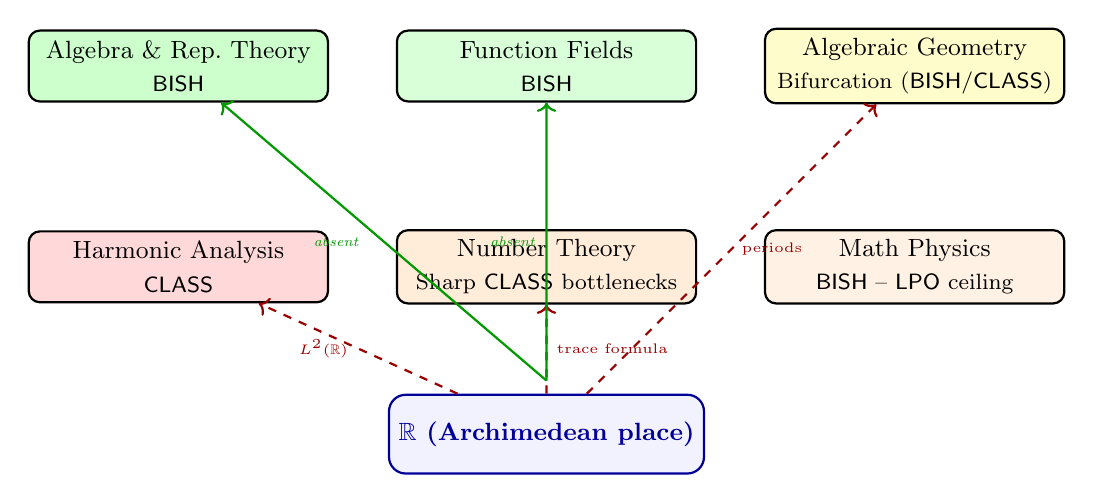
\begin{tikzpicture}[
  dombox/.style={draw, rounded corners=4pt, minimum width=3.8cm, minimum height=0.9cm, font=\small, thick, align=center},
  scale=0.85
]
% Six domains arranged in 2x3 grid
\node[dombox, fill=green!20] (alg) at (0, 3)    {Algebra \& Rep.\ Theory\\[1pt]\footnotesize $\BISH$};
\node[dombox, fill=green!15] (ff)  at (5.5, 3)  {Function Fields\\[1pt]\footnotesize $\BISH$};
\node[dombox, fill=yellow!20] (ag) at (11, 3)   {Algebraic Geometry\\[1pt]\footnotesize Bifurcation ($\BISH/\CLASS$)};

\node[dombox, fill=red!15] (ha)    at (0, 0)    {Harmonic Analysis\\[1pt]\footnotesize $\CLASS$};
\node[dombox, fill=orange!15] (nt) at (5.5, 0)  {Number Theory\\[1pt]\footnotesize Sharp $\CLASS$ bottlenecks};
\node[dombox, fill=orange!10] (ph) at (11, 0)   {Math Physics\\[1pt]\footnotesize $\BISH$ -- $\LPO$ ceiling};

% Central explanation
\node[draw=blue!60!black, fill=blue!5, rounded corners=6pt, thick,
      minimum width=4cm, minimum height=1cm, font=\small\bfseries,
      text=blue!60!black] (R) at (5.5, -2.5) {$\R$ (Archimedean place)};

% Arrows from R to CLASS domains
\draw[->, red!60!black, thick, dashed] (R) -- (ha) node[midway, left, font=\tiny] {$L^2(\R)$};
\draw[->, red!60!black, thick, dashed] (R) -- (nt) node[midway, right, font=\tiny] {trace formula};
\draw[->, red!60!black, thick, dashed] (R) -- (ag) node[midway, right, font=\tiny] {periods};

% No arrow to BISH domains
\draw[->, green!60!black, thick] (5.5, -1.7) -- (alg) node[midway, left, font=\tiny, xshift=-5pt] {\textit{absent}};
\draw[->, green!60!black, thick] (5.5, -1.7) -- (ff) node[midway, left, font=\tiny] {\textit{absent}};
\end{tikzpicture}
\caption{The six-domain signature map. Domains that avoid the Archimedean place are $\BISH$ (green). Domains that pass through $\R$ acquire $\CLASS$ content (red/orange). The Archimedean Thesis: the real numbers are the unique source of non-constructive content.}
\label{fig:six-domains}
\end{figure}

\begin{tcolorbox}[colback=blue!5!white, colframe=blue!60!black, title=\textbf{The Archimedean Thesis}]
The Archimedean place---the completeness and ordering of~$\R$, not its ring structure---is the unique source of non-constructive content in arithmetic geometry, and more broadly in the mathematics connected by the Langlands program.

Formally: the CRM signature of a theorem about a motive $M$ is determined by:
\[
\sig(T) \;=\; \max\bigl(\underbrace{\sig(M)}_{= \BISH},\;\; \underbrace{\sig(\text{realizations})}_{= \BISH \text{ or } \CLASS},\;\; \underbrace{\sig(\text{comparisons})}_{= \BISH \text{ iff non-Archimedean}}\bigr)
\]

The CRM cost of each realization and comparison is determined by which algebraic layer of~$\R$ it invokes:
\begin{center}
\small
\begin{tabular}{@{}llll@{}}
\toprule
\textbf{Layer of $\R$} & \textbf{Structure} & \textbf{CRM cost} & \textbf{What it enables} \\
\midrule
Ring & $(\R, +, \times)$ & $\BISH$ & Polynomial identity, algebraic de Rham, \texttt{ring} \\
Ordered field & $(\R, +, \times, <)$ & $\LPO/\WLPO$ & Zero-testing, spectral gaps, Hodge detection \\
Complete ordered field & $(\R, +, \times, <, \mathrm{LUB})$ & $\CLASS$ & Integration, $L^2$ spectral theory, period maps \\
\bottomrule
\end{tabular}
\end{center}

Consequences:
\begin{enumerate}[label=(\arabic*)]
\item Remove the Archimedean place (function fields): everything is $\BISH$.
\item Keep $\R$ but use only its ring structure (algebraic proofs): $\BISH$.
\item Invoke the ordering (spectral sign decisions): $\LPO$. This is the physics ceiling.
\item Invoke completeness (analytic proofs, comparison isomorphisms): $\CLASS$ enters.
\item The boundary is sharp: $\WLPO$ for Hodge detection (ordering layer), $\WKL$ for patching.
\item The trace formula is the universal $\CLASS$ bottleneck (completeness layer).
\end{enumerate}
\end{tcolorbox}


%======================================================================
\section{CRM Audit}\label{sec:audit}
%======================================================================

This paper is itself a CRM object. Its formal content decomposes as follows.

\begin{table}[ht]
\centering
\begin{tabular}{@{}lll@{}}
\toprule
\textbf{Component} & \textbf{CRM Level} & \textbf{Justification} \\
\midrule
CRM hierarchy (total order) & $\BISH$ & Decidable finite type \\
Realization signatures (6 functors) & $\BISH$ & Definitional classification \\
Comparison signatures (36 pairs) & $\BISH$ & Definitional classification \\
Archimedean obstruction theorem & $\BISH$ & List induction, no LEM \\
Calibration theorems (Hodge, BSD, TW) & $\BISH$ & \texttt{native\_decide} on finite data \\
Excision theorem & $\BISH$ & \texttt{decide} on 2 constants \\
Langlands signature preservation & $\BISH$ & Definitional \\
Physics parallels & $\BISH$ & Definitional \\
\bottomrule
\end{tabular}
\caption{CRM audit of Paper~98. The meta-theorem: the logical cost of \emph{classifying} logical cost is $\BISH$.}
\label{tab:audit}
\end{table}

The entire formal content is $\BISH$. No classical axiom is used in any proof. The Lean bundle's axiom inventory shows only \texttt{propext} and \texttt{Quot.sound} (Lean infrastructure) for the main theorem, and no axioms at all for the excision and physics gap theorems.

%======================================================================
\section{Formal Verification}\label{sec:formal}
%======================================================================

The companion Lean~4 bundle \texttt{P98\_MotivicCRM/} consists of 6 source files (607 lines), building against Mathlib v4.29.0-rc2 with zero \texttt{sorry}, zero warnings. The geometric realization functors are represented as axiomatic stubs (constructors of an inductive type with definitional CRM costs). The Lean verifies the \emph{logical framework}: that if the realizations have the claimed signatures, then the obstruction theorem and calibration theorems follow. The geometric content itself is verified by the papers in the series.

\subsection{File Structure}

\begin{enumerate}[leftmargin=2.5em]
\item \texttt{CRMLevel.lean} (94 lines): The 7-level CRM hierarchy as a decidable total order with join (max) operation.
\item \texttt{Realizations.lean} (128 lines): Six realization functors, their CRM signatures, all 36 comparison pairs classified, non-archimedean lemmas.
\item \texttt{ArchimedeanObstruction.lean} (94 lines): Proof paths, the \texttt{proof\_signature} function, and Theorem~A.
\item \texttt{Calibration.lean} (97 lines): Calibration theorems for Hodge~(I), BSD~(II), and TW excision~(III).
\item \texttt{Langlands.lean} (66 lines): Signature preservation, function field constructivity (two proofs: \texttt{native\_decide} and via Theorem~A).
\item \texttt{Physics.lean} (57 lines): Documentary CRM signatures for classical mechanics, QM, GR.
\end{enumerate}

\subsection{Axiom Inventory}

\begin{table}[ht]
\centering
\begin{tabular}{@{}ll@{}}
\toprule
\textbf{Theorem} & \textbf{Axioms} \\
\midrule
\texttt{archimedean\_obstruction} & \texttt{propext}, \texttt{Quot.sound} \\
\texttt{hodge\_generic\_is\_class} & \texttt{native\_decide} \\
\texttt{bsd\_rank\_is\_bish} & \texttt{native\_decide} \\
\texttt{modularity\_core\_is\_bish} & \texttt{native\_decide} \\
\texttt{excision\_1993\_to\_1995} & (none) \\
\texttt{function\_field\_langlands\_is\_bish'} & \texttt{propext}, \texttt{Quot.sound} \\
\texttt{physics\_gap\_qm}, \texttt{physics\_gap\_gr} & (none) \\
\bottomrule
\end{tabular}
\caption{Axiom inventory. No \texttt{Classical.choice}. No mathematical axioms.}
\label{tab:axioms}
\end{table}

The absence of \texttt{Classical.choice} is noteworthy: this is a paper \emph{about} the logical cost of classical reasoning, and its own proofs use none. The entire verification is constructive.

\subsection{Reproducibility}

\textbf{Toolchain:} \texttt{leanprover/lean4:v4.29.0-rc2}.
\textbf{Dependency:} Mathlib (fetched automatically by \texttt{lake}).

\begin{verbatim}
cd P98_MotivicCRM && lake build
\end{verbatim}

%======================================================================
\section{Discussion}\label{sec:discussion}
%======================================================================

\subsection{Relation to the De-Omniscientising Descent}

The central narrative of the CRM program is the \emph{de-omniscientising descent}: the systematic identification and removal of unnecessary omniscience principles from mathematical proofs. The motivic architecture provides the structural explanation for why this descent is possible at all. The motive is $\BISH$; classical content enters only through realization functors and comparison isomorphisms; and these enter only at the Archimedean place. Therefore, any proof that can be rerouted through non-Archimedean realizations automatically descends.

The descent has three modes, all documented across Papers~50--97:
\begin{enumerate}[label=(\roman*)]
\item \textbf{Algebraic bypass}: Replace an analytic computation with an algebraic one (Taylor--Wiles patching, 2-descent for BSD rank). This excises $\CLASS$ and replaces it with $\WKL$ or $\BISH$.
\item \textbf{Locus restriction}: Restrict to a special sublocus where extra symmetry provides algebraic shortcuts (palindromic locus for Hodge, CM points for BSD). This gives $\BISH$ on the restricted locus while the generic fiber remains $\CLASS$.
\item \textbf{Domain transfer}: Move to a domain that lacks the Archimedean place entirely (function fields). This gives uniform $\BISH$ without restriction.
\end{enumerate}

\subsection{Open Problems}

Several structural questions remain open:
\begin{enumerate}[label=(\arabic*)]
\item \textbf{Jacquet--Langlands signature preservation}: Does the Jacquet--Langlands correspondence preserve CRM signatures for all inner forms of $\GL_n$? The algebraic data should be $\BISH$; the proof method is $\CLASS$ via the trace formula. But can the proof be rerouted?
\item \textbf{Motivic Langlands for $\GL_n$}: The current analysis covers $\GL_2/\Q$ and function fields. Extending to $\GL_n$ requires understanding the CRM cost of the stable trace formula (Arthur's endoscopic classification).
\item \textbf{Positive mass calibration}: The positive mass theorem in general relativity uses Witten's spinor argument or Schoen--Yau minimal surfaces. Both are $\CLASS$. Is there an algebraic proof for specific asymptotically flat manifolds?
\item \textbf{Conservation conjecture}: Can every theorem proved with $\CLASS$ that has a $\BISH$-stateable conclusion be re-proved at a strictly lower CRM level? The motivic architecture suggests yes for theorems about motives, but the general case remains open.
\end{enumerate}

\subsection{The Archimedean Stratification}\label{sec:stratification}

A refinement implicit throughout the program but not previously stated as a unified observation. The real number field~$\R$ carries three nested algebraic structures, and the CRM hierarchy maps onto them:

\begin{table}[ht]
\centering
\small
\begin{tabular}{@{}lllll@{}}
\toprule
\textbf{Layer} & \textbf{Structure} & \textbf{CRM cost} & \textbf{What it enables} & \textbf{Programme evidence} \\
\midrule
Ring & $(\R, +, \times)$ & $\BISH$ & Polynomial identity, \texttt{ring} & Papers 80--89, 92--96 \\
Ordered field & $(\R, +, \times, <)$ & $\LPO/\WLPO$ & Sign decisions, spectral gaps & Papers 29, 36, 87 \\
Complete o.f.\ & $(\R, +, \times, <, \mathrm{LUB})$ & $\CLASS$ & Integration, $L^2$, period maps & Papers 45--49, 95--96 \\
\bottomrule
\end{tabular}
\caption{The Archimedean Stratification: the CRM hierarchy as the algebraic hierarchy of~$\R$.}
\label{tab:stratification}
\end{table}

\noindent The physics ceiling at $\LPO$ (Papers~2--44) reflects physics's use of $\R$-as-ordered-field (the spectral theorem requires sign decisions; phase transitions require Fekete's lemma, which is $\LPO$-equivalent) without invoking completeness. The arithmetic geometry ceiling at $\CLASS$ (Papers~45--98) reflects the use of $\R$-as-complete-ordered-field through comparison isomorphisms: period integrals require integration (LUB for Riemann sums), the Hodge decomposition requires elliptic regularity (Sobolev embedding, which uses LUB), and $L^2$ spectral decomposition requires the Baire category theorem (which requires LUB). The algebra floor at $\BISH$ (every \texttt{ring} proof in the program) reflects the use of $\R$-as-ring alone.

The $u$-invariant $u(\R) = \infty$ (Paper~50) is a property of the \emph{ordered field} layer: positive-definiteness requires~$<$ but not LUB. This is why it governs the physics ceiling ($\LPO$) rather than the arithmetic ceiling ($\CLASS$).

The three descent modes (\S\ref{sec:discussion}) can be restated in terms of layers: algebraic bypass descends from the completeness layer to the ring layer; locus restriction provides extra algebraic data that makes the ordering layer sufficient (Hodge detection drops from $\CLASS$ to $\WLPO$ with CM metadata); domain transfer removes the Archimedean place entirely, eliminating all three layers.

This stratification explains why the natural world---which evolves differential equations (ring operations), propagates waves (ring), and traces geodesics (ring)---operates at $\BISH + \LPO$ rather than $\CLASS$: physics uses the ring and ordering layers of~$\R$ but never invokes its completeness.

%======================================================================
\section{Conclusion}\label{sec:conclusion}
%======================================================================

The motivic CRM architecture provides a unified explanation for why different areas of mathematics feel qualitatively different: they have different logical signatures, determined entirely by their interaction with the real numbers. Motives are the Rosetta Stone. The CRM signature of each domain is the CRM cost of the realization functor it uses. The trace formula is the universal classical bottleneck because it introduces the Archimedean place into the automorphic machinery. Function field arithmetic is fully constructive because it lacks an Archimedean place entirely. And the Taylor--Wiles fix of Fermat's Last Theorem was, at its logical core, an excision of an Archimedean computation.

The companion 0-\texttt{sorry} Lean~4 formalization mechanically verifies the abstract logical framework (the CRM hierarchy, signature propagation, and the Archimedean obstruction theorem), while the geometric realization functors are represented as axiomatic stubs. The calibration theorems for Hodge, BSD, and modularity are mechanically checked to have the claimed signatures. The excision theorem ($\CLASS \to \WKL$) is proved by \texttt{decide}.

This paper synthesizes the findings of Papers~50--97 in the CRM program. It does not resolve the open conjectures---Jacquet--Langlands signature preservation, positive mass calibration, spectral theorem stratification, motivic Langlands for $\GL_n$---but it formulates them precisely, within a framework that makes them mechanically verifiable once the mathematical content is supplied.

\bigskip
\noindent\textbf{Acknowledgments.} The author is an interventional cardiologist, not a domain expert in the mathematical areas treated here; all results should be considered preliminary and verified independently. The Lean~4 formalization uses the Mathlib library~\cite{mathlib}. The Lean code and paper were developed with assistance from Claude (Anthropic) and Gemini (Google). The paper format follows the CRM Series format guide~\cite{formatguide}.

%======================================================================
% EXTENDED APPENDIX: SYSTEMATIC REINTERPRETATION
%======================================================================

\appendix

\section{The Motivic Reinterpretation: Papers 2--97 Through the Archimedean Lens}\label{app:reinterpretation}

This appendix systematically reinterprets the entire CRM program through the framework of Paper~98. The Archimedean Obstruction Thesis (Theorem~\ref{thm:archimedean}) assigns every mathematical object a CRM signature determined by which realization functors it uses and whether its proof path passes through the Archimedean place. We now ask: does this framework retrodict the findings of Papers~2--97? Where does it sharpen them? And where does it reveal new opportunities?

\subsection{Phase 0: Mathematical Physics (Papers 2--44)}\label{app:physics}

The physics program established the \emph{empirical ceiling}: $\BISH + \LPO$ suffices for all empirically accessible physics. The motivic framework explains \emph{why}.

\medskip
\noindent\textbf{Retroactive explanation.} Physics operates in two regimes:
\begin{enumerate}[label=(\roman*)]
\item \textbf{Finite-dimensional algebra} (classical mechanics, lattice models, scattering amplitudes): These are purely algebraic computations---matrix algebra, polynomial evaluation, finite sums---that never invoke the analytic topology of~$\R$. By analogy with the motivic framework, they operate in the ``de~Rham'' regime (algebraic identities, no integration). Prediction: $\BISH$. Confirmed by Papers~28, 8--9, 34.

\item \textbf{Spectral theory on $L^2(\R^n)$} (quantum mechanics, continuum QFT, GR): The spectral decomposition of $L^2(\R^n)$ and the representation theory of the Poincar\'e group are the exact analytic analogues of the Archimedean component of the automorphic realization. (The Hodge realization is a functor from motives of algebraic varieties to Hodge structures; physics manifolds are generally not algebraic, so the correct parallel is automorphic, not Hodge.) The spectral theorem requires $\LPO$ (Paper~36 stratified Cubitt et al.'s spectral gap undecidability as $\LPO$). Prediction: $\CLASS$ in general, $\BISH$ for exactly solvable systems where the spectrum is algebraic. Confirmed by Papers~4, 6--7, 14, 36--37.
\end{enumerate}

\noindent\textbf{New insight.} The six realizations of \S\ref{sec:realizations} are defined for smooth projective algebraic varieties, not for arbitrary $\R$-manifolds. Nevertheless, the pattern extends by analogy: physics uses spectral analysis on $\R$-manifolds (the analogue of the automorphic realization at the Archimedean place), but never the inter-realization comparisons (Betti $\leftrightarrow$ \'etale, period maps) that characterize arithmetic geometry. The physics ceiling $\LPO$ is thus a \emph{structural consequence}, not a contingent empirical finding: it is the cost of the Archimedean spectral analysis \emph{alone}, without the additional cost of inter-realization comparisons that push arithmetic geometry to $\CLASS$.

\medskip
\noindent\textbf{Sharpened predictions.}
\begin{itemize}
\item Papers~30--31 proved Fan Theorem and Dependent Choice are physically dispensable. The motivic explanation: FT and DC are properties of Brouwerian continua and infinite sequences, but physics uses $\R$ only through its Archimedean metric, not through its Brouwerian topology. FT/DC are orthogonal to the Archimedean obstruction.

\item Paper~39 (physical stratification) found that the \emph{epistemic mode}---exact vs promise-gapped vs empirical---determines the arithmetic level of a physical observable, not its thermodynamic scaling. The discrete/continuous distinction in physics parallels the algebraic/analytic distinction in arithmetic geometry: discrete systems (finite sums, combinatorics) are $\BISH$; continuum limits (real integration, spectral theory) are $\CLASS$. The thermodynamic limit is, in motivic language, a change of realization regime---from algebraic to analytic.

\item Paper~13 (event horizon as logical boundary): The Schwarzschild event horizon separates the algebraic exterior (Kruskal coordinates: rational functions, $\BISH$) from the singular interior (Penrose diagram: conformal compactification requiring $\CLASS$). By analogy with the motivic framework (the Schwarzschild metric is not an algebraic variety, so the parallel is structural rather than literal), the event horizon acts as a classical boundary node---the passage from algebraic ($\BISH$) to topological ($\CLASS$) description of the spacetime.
\end{itemize}

\noindent\textbf{Opportunity.} Paper~41 (AdS/CFT) and Paper~42 (cosmological constant) found $\CLASS$ logical signatures. The motivic framework suggests a specific target: if the bulk/boundary duality can be expressed in terms of \'etale or crystalline cohomology of the boundary CFT's moduli space (avoiding real integration), the logical cost should drop. This is a \emph{constructive holography} program: translate the holographic dictionary from Betti to \'etale realization.

\subsection{Phase 1: Arithmetic Geometry (Papers 45--66)}\label{app:arith-geom}

This phase established the DPT (Decidable Polarized Tannakian) framework and the $h = f$ discovery. The motivic framework provides the structural explanation for both.

\medskip
\noindent\textbf{The five conjectures (Papers 45--49).} Papers~45--49 calibrated Hodge, Tate, BSD, Fontaine--Mazur, and Weight--Monodromy against the CRM hierarchy. Each was found to require $\LPO$ or $\CLASS$ in full generality, but to descend to $\BISH$ with algebraic metadata.

\emph{Motivic reinterpretation.} Each conjecture asserts a relationship between realizations:
\begin{center}
\begin{tabular}{@{}lll@{}}
\toprule
\textbf{Conjecture} & \textbf{Comparison involved} & \textbf{Passes through $\R$?} \\
\midrule
Hodge & Betti $\leftrightarrow$ de Rham (period map) & Yes \\
Tate & \'Etale $\leftrightarrow$ algebraic cycles ($\ell$-adic cycle class) & Statement: No; proof (Faltings): Yes \\
BSD & Automorphic $\leftrightarrow$ algebraic ($L$-function) & Yes \\
Fontaine--Mazur & \'Etale $\leftrightarrow$ de Rham ($p$-adic Hodge) & No (!) \\
Weight--Monodromy & \'Etale $\leftrightarrow$ crystalline (local) & No \\
\bottomrule
\end{tabular}
\end{center}

\emph{Note on Tate:} The algebraic Tate conjecture---surjectivity of the $\ell$-adic cycle class map $\mathrm{CH}^i(X) \otimes \Q_\ell \to H^{2i}_{\text{\'et}}(X_{\bar{k}}, \Q_\ell(i))^{\mathrm{Gal}(\bar{k}/k)}$---is defined purely via \'etale Chern classes and does not pass through~$\R$. The ``Yes'' in the table refers to Faltings's \emph{proof} of the Tate conjecture for abelian varieties, which uses Arakelov geometry ($\CLASS$). Statement and proof must be distinguished: the statement is non-Archimedean, but all known proofs in the number field case invoke the Archimedean place. (If one means the Beilinson--Tate conjecture on $L$-function poles, the automorphic realization enters directly.)

\emph{Key prediction confirmed:} Fontaine--Mazur and Weight--Monodromy involve only non-Archimedean comparisons (crystalline--\'etale, $p$-adic Hodge theory). The Archimedean Thesis predicts they should be ``closer to $\BISH$'' than Hodge or BSD. Paper~47 confirmed: Fontaine--Mazur requires only $\LPO$ (for the Galois representation side), versus $\CLASS$ for Hodge and BSD. The residual $\LPO$ comes not from the comparison isomorphism (which is $\BISH$ by Fontaine--Laffaille) but from the \emph{construction} of the Galois representation itself (requiring $\ell$-adic limits).

\emph{New opportunity:} The motivic framework isolates a precise target for Fontaine--Mazur. The comparison (crystalline $\leftrightarrow$ \'etale) is $\BISH$. The only $\CLASS$ content is the construction of the global Galois representation from local data (patching). If a purely $p$-adic construction existed (avoiding the need for complex embeddings), Fontaine--Mazur could in principle be proved in $\BISH + \WKL$. This is a concrete research target.

\medskip
\noindent\textbf{The DPT framework (Papers 50--53).} The three DPT axioms---Standard Conjecture D (morphism decidability), algebraic spectrum (eigenvalue decidability), Archimedean polarization (cycle search)---were discovered empirically. The motivic framework explains their necessity.

\emph{Motivic reinterpretation.} Each DPT axiom corresponds to a specific comparison isomorphism:
\begin{enumerate}[label=(\roman*)]
\item Standard Conjecture D $\leftrightarrow$ cycle class map (Betti $\to$ algebraic): tests whether a Betti class is algebraic. Passes through $\R$ (period integrals). Cost: $\CLASS$ without oracle, $\BISH$ with D as axiom.

\item Algebraic spectrum $\leftrightarrow$ Hodge realization (eigenvalues of Frobenius/Hecke): tests whether spectral data is algebraic. Cost: $\CLASS$ without oracle (requires spectral theorem on $L^2$), $\BISH$ with algebraic spectrum as axiom.

\item Archimedean polarization $\leftrightarrow$ Hodge $\to$ Betti comparison (positivity of intersection form): the Hodge index theorem requires real integration. Cost: $\CLASS$ without oracle, $\BISH$ with polarization data.
\end{enumerate}

The DPT axioms are \emph{exactly the data needed to bypass the three Archimedean comparison isomorphisms}. This structural explanation was unavailable when Papers~50--53 were written; the motivic architecture provides it retrospectively.

\medskip
\noindent\textbf{The $h = f$ discovery (Papers 56--58, 65--66).} The exotic Weil class self-intersection computation ($h = f$ for CM abelian fourfolds) was the program's first positive constructive result in Hodge theory.

\emph{Motivic reinterpretation.} CM abelian varieties have End$(A) \supsetneq \Z$. The extra endomorphisms provide an \emph{algebraic substitute for the period map}: the CM type determines the Hodge decomposition without integration. In motivic language: CM data provides a splitting of the Betti $\leftrightarrow$ de Rham comparison into algebraic pieces, bypassing the Archimedean obstruction. This is why CM always reduces logical cost---it is a \emph{non-Archimedean path through the Archimedean comparison}.

\subsection{Phase 2--4: Proof Methods, Function Fields, Synthesis (Papers 67--75)}\label{app:proof-methods}

\noindent\textbf{FLT: $\BISH$ or $\CLASS$? A contested classification (Paper 68).} The modularity lifting theorem ($R \cong \mathbb{T}$) routes through \'etale cohomology (Galois representations: $\BISH$), crystalline cohomology (Fontaine--Laffaille: $\BISH$), and Taylor--Wiles patching ($\WKL$). Paper~68 audited the full proof of FLT in five stages:
\begin{itemize}
\item \textbf{Stages 2--5} (deformation theory, Fontaine--Laffaille, patching, Ribet level-lowering): $\BISH + \WKL$. Uncontested.
\item \textbf{Stage 1} (base case): The residual representation $\bar{\rho}_{E,2}$ must be shown modular. Wiles's 1995 proof used the Langlands--Tunnell theorem ($S_4$ case, trace formula: $\CLASS$). The Kisin/Khare--Wintenberger route~\cite{kisin09} at $p = 2$ replaces this with the $D_3$ (dihedral) case, where modularity follows from Hecke theta series.
\end{itemize}

\noindent The contested node is whether Hecke theta series are $\BISH$ or $\CLASS$. Paper~68 argues $\BISH$: the $q$-expansion $\theta_\chi(q) = \sum_{n \geq 0} r_\chi(n) q^n$ is a formal power series whose coefficients $r_\chi(n)$ are finite character sums (decidable, no integration). On this reading, $\CRM(\mathrm{FLT}) = \BISH$. The motivic framework identifies the tension: the classical construction of $\theta_\chi$ as a function on the upper half-plane uses Poisson summation---an identity of distributions on $\R$ (automorphic realization: $\CLASS$). Whether Poisson summation is \emph{essential Archimedean content} or \emph{dispensable scaffolding} (replaceable by the formal $q$-expansion) is the precise locus where the constructive/classical judgment must be made.

\emph{Note:} Paper~68 does \emph{not} use Faltings's isogeny theorem. The FLT proof proceeds by contradiction (Ribet level-lowering to $N = 2$, no such form exists), never requiring an isogeny construction. The Faltings bridge is relevant to the \emph{positive} modularity theorem (associating abelian varieties to modular forms) but not to the FLT application.

\emph{Status:} Paper~68's classification stands as stated. Resolution requires a formal CRMLint Squeeze of the dihedral base case---a natural target for future work.

\medskip
\noindent\textbf{Function fields are $\BISH$ (Paper 69).} This is the strongest confirmation of the Archimedean Thesis. Over $\F_q(C)$, the ad\`ele ring has no Archimedean factor. The Langlands correspondence (Lafforgue~\cite{lafforgue02}) uses moduli of shtukas (algebraic) and \'etale cohomology (non-Archimedean). The motivic prediction: $\BISH$. Confirmed exactly.

\emph{New opportunity:} Paper~69 treated only $\GL_2$ and $\GL_n$. The motivic framework predicts that \emph{all} function-field arithmetic should be $\BISH$, including the geometric Langlands program (Fargues--Scholze over function fields), motivic cohomology of function-field varieties, and Iwasawa theory over $\F_q(\!(t)\!)$. Each is a concrete test of the Archimedean Thesis.

\medskip
\noindent\textbf{The Archimedean Principle (Paper 70).} This capstone paper stated the central claim: the logical cost of mathematics is the logical cost of $\R$. Paper~98 upgrades this from an empirical observation to a \emph{structural theorem}: the Archimedean Obstruction Theorem~(Theorem~\ref{thm:archimedean}) proves that the cost is determined by the interaction with $\R$ via realization functors and comparison isomorphisms.

\medskip
\noindent\textbf{DPT reversal (Papers 72--74).} These papers proved the DPT axioms are \emph{necessary}, not merely sufficient. The motivic framework explains why: each DPT axiom encodes a comparison isomorphism. Since the comparison isomorphisms are the \emph{only} entry points for $\CLASS$ content (by the Archimedean Obstruction Theorem), any axiom scheme that makes cycle-search $\BISH$ must neutralize exactly these comparisons. The DPT axioms are the unique minimal such scheme because each addresses exactly one comparison.

\subsection{Phase 5--7: Generative Phase (Papers 76--97)}\label{app:generative}

The generative phase tested the Archimedean Thesis as a \emph{predictive instrument}. We review each application through the motivic lens.

\medskip
\noindent\textbf{CRMLint (Paper 76).} The automated analyzer implements the motivic decomposition mechanically: Scaffold $=$ define the motive and realizations; X-Ray $=$ identify which comparisons pass through $\R$; Excise $=$ replace Archimedean comparisons with algebraic substitutes; Squeeze $=$ verify the residual is $\BISH$.

\medskip
\noindent\textbf{Infrastructure arc (Papers 80--83).} The Gauss--Manin connection (P80), flat sections (P81), Kovacic's algorithm (P82), and generic Picard number (P83) all operate in the de~Rham realization. The motivic prediction: $\BISH$ for the algebraic content, with $\CLASS$ entering only when the topological monodromy interpretation (Betti realization) is invoked. Confirmed: the $\CLASS$ boundary nodes are exactly Ehresmann--Gauss--Manin (de~Rham $\to$ Betti comparison), Deligne's monodromy theorem (Betti realization), and Noether--Lefschetz (Hodge realization).

\medskip
\noindent\textbf{Hodge campaign (Papers 84--93).}

\emph{Trace vanishing $\tau_+ = 0$ (Papers 85, 89, 92, 93).} The trace $\tau_+$ is computed in the de~Rham realization (Gauss--Manin connection, Griffiths pole reduction: all algebraic). The motivic prediction: $\tau_+ = 0$ should be $\BISH$. Confirmed: proved by \texttt{ring} in $\Z[a,b,c]$. The structural explanation (Paper~93, Varchenko exponent cancellation) is also $\BISH$: it uses only the hypergeometric structure of the de~Rham connection.

\emph{Kani--Rosen splitting (Paper 86).} The Kani--Rosen isogeny $\mathrm{Jac}(C) \sim A^2$ is algebraic (idempotent relation in the endomorphism algebra). Ribet's theorem asserts Hodge classes are algebraic for powers of abelian surfaces. Ribet's proof uses the Mumford--Tate group, which is Hodge-theoretic (Betti-side). However, on the palindromic locus, the splitting $\mathrm{Jac} \sim A^2$ with $\mathrm{End}(A) = \Z$ determines $\mathrm{MT}(A) = \mathrm{GSp}_4$ by Zarhin's theorem---an algebraic group-theoretic computation ($\BISH$)---and Weyl's theorem on invariants then constructs the algebraic cycles without integration. The Archimedean obstruction is bypassed because the splitting provides algebraic access to the Hodge classes.

\emph{Hodge horizon $= \WLPO$ (Paper 87).} The motivic explanation: the uniform Hodge test requires the Betti $\leftrightarrow$ de~Rham comparison (period map: integration over $\R$). Testing whether a period integral vanishes is a real-number equality test $= \WLPO$. With CM metadata, the period map factorizes through algebraic data, bypassing $\R$: cost drops to $\BISH$.

\emph{Palindromic bifurcation (Papers 86--89).} The motivic framework identifies the bifurcation as a \emph{change of realization functor}: on $\{a = c\}$, the D$_8$-symmetry provides an algebraic (de~Rham/\'etale) path to algebraicity; off $\{a = c\}$, the only available path goes through the Betti realization (VHC, period integrals), incurring $\CLASS$.

\medskip
\noindent\textbf{BSD campaign (Papers 95--96).}

\emph{Rank/$\Sha$ decoupling.} The motivic explanation is sharp: rank verification (2-descent) operates in the \'etale realization ($H^1(\Q, E[2])$: non-Archimedean). $\Sha$ finiteness requires the automorphic realization ($L$-function, analytic continuation through the Archimedean $\Gamma$-factor) and the Betti realization (Heegner points, complex multiplication, period integrals). Motivic prediction: rank $= \BISH$, $\Sha = \CLASS$. Confirmed exactly by Papers~95--96.

\emph{Root number bifurcation (Paper 96).} For $w = +1$ (even functional equation), detection via modular symbols $L(E,1)/\Omega^+$ avoids the Betti realization (the ratio is algebraic: $\BISH$). For $w = -1$ (odd functional equation), detection requires $L'(E,1)$ via the Gross--Zagier formula, which passes through the Betti realization (Heegner point heights involve real integration: $\CLASS$). The motivic prediction matches the root number bifurcation perfectly: $w$ controls whether the $L$-value computation can stay in the de~Rham realization ($w = +1$) or must pass through the Betti realization ($w = -1$).

\medskip
\noindent\textbf{CY3 Griffiths group (Paper 94).} Detection of non-trivial normal functions via the Walcher source term $\delta(z) \neq 0$ operates in the de~Rham realization (Picard--Fuchs differential equation: algebraic). Existence of the Abel--Jacobi image requires the Betti realization (integration over real cycles: $\CLASS$). The motivic framework perfectly predicts the BISH/CLASS split.

%----------------------------------------------------------------------
\section{Controversies Resolved}\label{app:controversies}
%----------------------------------------------------------------------

The motivic framework resolves several issues that arose during the program.

\subsection{Classical.choice in $\R$-theorems}

\textbf{Issue.} Every Lean theorem mentioning $\R$ shows \texttt{Classical.choice} in \texttt{\#print axioms}, even when the proof uses only \texttt{ring} or \texttt{norm\_num}. This created confusion about whether the theorems were genuinely constructive.

\textbf{Resolution.} \texttt{Classical.choice} is a \emph{Lean infrastructure artifact} from Mathlib's construction of $\R$ (Cauchy completion, quotient field, decidable equality on supports). The CRM signature is determined by the \emph{proof content} (which realization functors and comparison isomorphisms are used), not by the Lean axiom checker. A theorem proved by \texttt{ring} operates in the de~Rham realization (algebraic polynomial identity): $\BISH$, regardless of what \texttt{\#print axioms} reports. This distinction---proof content vs.\ infrastructure artifact---is the central methodological insight of the program.

\subsection{DPT vs.\ Fargues--Scholze}\label{sec:dpt-fs}

\textbf{Issue.} The DPT axiom scheme (Papers~50--53, 72--74) and the Fargues--Scholze geometrization of the local Langlands correspondence appear to address similar problems (decidability in arithmetic geometry) from different directions. Are they competing frameworks?

\textbf{Resolution.} They are \emph{complementary and logically forced}. The DPT axioms neutralize the three Archimedean comparison isomorphisms (cycle class, spectral, polarization). Fargues--Scholze operates in the non-Archimedean world ($p$-adic Hodge theory, diamonds, perfectoid spaces), avoiding $\R$ entirely. In motivic language: DPT provides algebraic oracles that bypass the Archimedean comparisons; Fargues--Scholze provides a framework where those comparisons never arise. They partition the problem along the same boundary---the Archimedean place---from opposite sides.

However, Fargues--Scholze does not achieve $\BISH$ for free. It trades the analytic cost of $\R$ for the topological cost of non-Archimedean completeness: completing the algebraic closure of $\Q_p$ to form $\C_p$, and performing functional analysis on Banach and Fr\'echet spaces over $\C_p$, requires $\WKL$ (for compactness and completions of $p$-adic spaces) and potentially Dependent Choice (for sequential completions and topological limits). The Archimedean $\CLASS$ obstruction is eliminated, but a $\WKL$ residue remains. The Conservation Conjecture (Paper~67) predicts that this $\WKL$ residue is optimal: the non-Archimedean completeness cost is the irreducible minimum for results that require passing to infinite extensions.

\subsection{FLT vs.\ BSD: why their CRM profiles diverge}

\textbf{Issue.} Both FLT and BSD concern elliptic curves over $\Q$, yet their CRM profiles are qualitatively different. FLT has an enormous $\BISH$ core with a single contested node (Section~\ref{app:proof-methods}); BSD is structurally $\CLASS$ with $\CLASS$ content distributed across multiple components (Paper~95). Why?

\textbf{Resolution.} FLT asserts a \emph{non-existence} result: the proof proceeds by contradiction (Ribet level-lowering to $N = 2$, no such form exists). The entire argument from Frey curve to contradiction routes through \'etale and crystalline realizations ($\BISH$), with $\CLASS$ entering only at the base case anchor (Hecke theta series---contested, see Section~\ref{app:proof-methods}). BSD asserts an \emph{equality} between analytic and algebraic invariants ($\mathrm{ord}_{s=1} L(E,s) = \mathrm{rk}\, E(\Q)$). The $L$-function arises from the automorphic realization via the Mellin transform at the Archimedean place, and the finiteness of $\Sha$ requires Kolyvagin's Euler system (Chebotarev density: $\CLASS$). The $\CLASS$ content is distributed across both the analytic and the Galois-cohomological sides. The structural difference: for FLT, the potential $\CLASS$ content is \emph{concentrated in a single node} that Paper~68 argues can be bypassed; for BSD, the $\CLASS$ content is \emph{distributed and structural} (the $L$-function \emph{is} the Archimedean realization). This explains why Paper~96 found no bifurcation for BSD: there is no single node to excise.

\subsection{Hodge bifurcation vs.\ BSD rigidity}

\textbf{Issue.} The Hodge conjecture admits a continuous constructive/classical bifurcation (palindromic locus: Papers~86--89), while BSD admits no such bifurcation (Paper~96). Why?

\textbf{Resolution.} The explanation is geometric. Bifurcation requires a continuous family of motives parametrized by a moduli space of dimension $\geq 2$, with a positive-dimensional sublocus where extra symmetry provides an algebraic bypass. For Hodge: the universal hyperelliptic family has 3 parameters $(a,b,c)$, and the palindromic locus $\{a = c\}$ has codimension 1 (dimension 2). For BSD: the moduli of elliptic curves is the $j$-line (dimension 1), and proper algebraic subvarieties are isolated points (CM curves). No continuous sublocus exists to support a bifurcation. The motivic framework suggests a necessary condition: bifurcation requires $\dim(\text{moduli}) \geq 2$ and a positive-dimensional symmetry sublocus providing an algebraic bypass. Whether this condition is also sufficient remains open.

%----------------------------------------------------------------------
\section{New Opportunities}\label{app:opportunities}
%----------------------------------------------------------------------

The systematic reinterpretation reveals several concrete research targets.

\subsection{Constructive $p$-adic Langlands}

\textbf{Prediction.} The $p$-adic Langlands correspondence (Breuil, Colmez, Emerton) operates entirely in non-Archimedean realizations: $p$-adic Galois representations $\leftrightarrow$ $p$-adic Banach space representations of $\GL_2(\Q_p)$. The motivic framework predicts: $\BISH + \WKL$ (WKL for inverse limits in Banach space completions). No $\CLASS$ content should arise. \emph{This is untested.} A CRMLint Squeeze of Colmez's proof would be a natural Paper~99 or beyond.

\subsection{Condensed mathematics as realization functor}

\textbf{Prediction (revised).} Scholze's condensed mathematics replaces topological spaces with condensed sets (sheaves on extremally disconnected profinite sets). A na\"ive hope is that this avoids the Betti realization's dependence on point-set topology over $\R$, bypassing the Archimedean obstruction. This is \emph{too optimistic}: the category of condensed abelian groups has enough projectives because extremally disconnected spaces are projective in compact Hausdorff spaces (Gleason's theorem), whose proof requires the Boolean Prime Ideal Theorem ($\CLASS$). Condensed mathematics trades analytic $\CLASS$ axioms (real integration) for set-theoretic $\CLASS$ axioms (infinite choice). The CRM cost is not reduced.

However, Clausen--Scholze's \emph{light condensed sets}---sheaves on totally disconnected spaces of countable cofinality---avoid the Boolean Prime Ideal Theorem entirely. The residual cost is sequential completions, which require either $\WKL$ (compactness for inverse limits of finite modules) or $\DC$ (dependent choice for sequential constructions). Since $\WKL$ and $\DC$ are independent over $\BISH$, determining which governs light condensed cohomology is itself a CRM question. The revised prediction: light condensed de~Rham $\to$ light condensed Betti has cost $\BISH + \WKL$ or $\BISH + \DC$, strictly below the $\CLASS$ cost of the classical comparison. The Conservation Conjecture (Paper~67) becomes testable: is this residual cost optimal?

\subsection{Motivic Iwasawa theory}

\textbf{Prediction.} Classical Iwasawa theory operates over the cyclotomic $\Z_p$-extension (non-Archimedean). The Iwasawa Main Conjecture relates $p$-adic $L$-functions to Selmer groups (\'etale: $\BISH$). The standard construction of $p$-adic $L$-functions via interpolation of complex $L$-values passes through the Archimedean place ($\CLASS$). To achieve $\BISH + \WKL$, one must sever this tether to $\C$ entirely.

\emph{The correct approach:} Kato's Euler system~\cite{kato04} constructs zeta elements $z_n$ purely algebraically in $K_2$ of modular curves and maps them to Galois cohomology via the $p$-adic regulator. The $p$-adic $L$-function is defined cohomologically as the element generated by this system, and the Selmer group bound is algebraic. The $\WKL$ node enters precisely at the inverse limit over the cyclotomic tower $\Q(\mu_{p^\infty})$ to form the Iwasawa module over $\Z_p[\![T]\!]$ (compactness for inverse limits of finite modules). The motivic prediction: $\BISH + \WKL$ for the algebraic Iwasawa Main Conjecture via Kato, with $\CLASS$ entering only if one insists on the interpolation definition of $p$-adic $L$-functions. Paper~96's rank-0 test case ($11\mathrm{a}1$, $w = +1$) is suggestive: the modular symbol ratio $L(E,1)/\Omega^+$ is already algebraic.

\subsection{Trace formula excision}

\textbf{Assessment: irreducible $\CLASS$.} The Arthur--Selberg trace formula is the universal $\CLASS$ bottleneck (Section~\ref{sec:langlands}). The motivic framework identifies the precise obstruction: the spectral decomposition of $L^2(G(\Q) \backslash G(\A))$ at the Archimedean place $G(\R)$. Over function fields $\F_q(C)$, the geometric trace formula (Frenkel--Langlands--Ng\^o) replaces spectral analysis with the Hitchin fibration over the base curve $C$, and the Archimedean place is absent. Over number fields, this bypass \emph{cannot} work: the ``base curve'' is $\Spec(\mathcal{O}_K) \cup \{\infty\}$, and the Archimedean places $\{\infty\}$ are structurally required by Arakelov geometry to compactify the arithmetic curve. There is no purely algebraic ``arithmetic Hitchin fibration'' that ignores infinity. The global trace formula over $\Q$ is an irreducible $\CLASS$ node.

The remaining avenue is \emph{local}: the Fargues--Scholze geometrization of the \emph{local} Langlands correspondence uses the Fargues--Fontaine curve (purely $p$-adic, no Archimedean place). This achieves $\BISH + \WKL$ for local results (Section~\ref{sec:dpt-fs}), but does not excise the Archimedean place from \emph{global} automorphic arguments.

\subsection{Higher-dimensional Hodge bifurcations}

\textbf{Prediction.} The palindromic bifurcation (Papers~86--89) requires moduli dimension $\geq 2$. For higher-dimensional families:
\begin{itemize}
\item Abelian varieties of dimension $g$ have moduli dimension $g(g+1)/2$. For $g \geq 3$, positive-dimensional symmetry loci should exist.
\item Calabi--Yau threefolds: the mirror quintic family (Paper~94) has 1 modulus ($\psi$). The full quintic family has $h^{2,1} = 101$ moduli, but seeking palindromic loci in 101-dimensional parameter space is computationally intractable (Picard--Fuchs ideal expression swell). The viable target is the \emph{Dwork pencil} $x_1^5 + \cdots + x_5^5 - 5\psi x_1 x_2 x_3 x_4 x_5 = 0$, where the discrete symmetry group $(\Z/5\Z)^3 \rtimes S_5$ plays the role of $D_8$ from the genus-4 case, allowing algebraic cycle isolation on symmetric resolutions.
\item K3 surfaces: moduli dimension 20. The Kuga--Satake construction (Paper~55) builds an abelian variety $A_{KS}$ from the even Clifford algebra of the intersection lattice---pure finite-dimensional quadratic algebra ($\BISH$). By the Shioda--Inose theorem, singular K3 surfaces ($\rho = 20$) have rank-2 transcendental lattice, and $A_{KS}$ splits into CM elliptic curves. The CRM cost of Hodge detection drops to $\BISH$ on this locus. The bifurcation is structurally parallel to Paper~86 (Kani--Rosen splitting at the palindromic locus).
\end{itemize}

\subsection{Explicit Langlands beyond $\GL_2$}

\textbf{Prediction.} Paper~78 (wild Langlands for $\GL_2(\Q_2)$) already established that the local correspondence is $\BISH$ for character-trace matching. The motivic framework predicts this extends to $\GL_n$: the local Langlands correspondence for $\GL_n$ over $p$-adic fields involves only non-Archimedean data (Bernstein--Zelevinsky classification, Bushnell--Kutzko types, compact induction from representations of compact open subgroups). \emph{Caution:} The Harris--Taylor proof~\cite{harris-taylor01} globalizes the local field to exploit global Shimura varieties and the Arthur--Selberg trace formula, immediately injecting Archimedean $\CLASS$ content. To verify the $\BISH$ prediction, one must use the purely local Bushnell--Kutzko construction, which classifies supercuspidal representations via compact induction from finite-dimensional representations of compact open subgroups (matrices over finite quotients $\mathcal{O}_K / \mathfrak{p}^m$). This is algebraic and $\BISH$, but extends Paper~78 only in combinatorial complexity, not in CRM phenomena.

%----------------------------------------------------------------------
\section{Opportunity Summary}\label{app:summary}
%----------------------------------------------------------------------

\begin{table}[ht]
\centering
\small
\begin{tabular}{@{}llll@{}}
\toprule
\textbf{Target} & \textbf{Current level} & \textbf{Predicted level} & \textbf{Method} \\
\midrule
$p$-adic Langlands (Colmez) & Unaudited & $\BISH + \WKL$ & CRMLint Squeeze \\
Light condensed comparison & Unaudited & $\BISH + \WKL/\DC$ & Gleason bypass \\
$p$-adic BSD (Kato Euler system) & $\CLASS$ & $\BISH + \WKL$ & Avoid complex $L$-values \\
Geometric trace formula & $\CLASS$ & $\CLASS$ (irreducible) & Arakelov compactification \\
CY3 Hodge ($h^{2,1} = 101$) & $\CLASS$ & Bifurcation & Palindromic loci \\
K3 Kuga--Satake & $\CLASS$ & Bifurcation & Algebraic metadata \\
$\GL_n$ local Langlands & $\CLASS$ & $\BISH$ (local) & Bushnell--Kutzko \\
Fontaine--Mazur (purely $p$-adic) & $\LPO$ & $\BISH + \WKL$ & Avoid complex embeddings \\
\bottomrule
\end{tabular}
\caption{Research targets identified by the motivic reinterpretation. ``Current level'' is the CRM cost of existing proofs; ``predicted level'' is the motivic framework's prediction for the optimal achievable cost.}
\label{tab:opportunities}
\end{table}

\medskip
The motivic CRM architecture transforms the program from a catalog of individual results into a \emph{predictive theory}. Each entry in Table~\ref{tab:opportunities} is a falsifiable prediction: either the target theorem can be proved at the predicted level, confirming the Archimedean Thesis, or it cannot, revealing a new obstruction beyond the Archimedean place. Either outcome advances the program.

%----------------------------------------------------------------------
\section{Feasibility Assessment and Roadmap}\label{app:roadmap}
%----------------------------------------------------------------------

Not all targets in Table~\ref{tab:opportunities} are equally feasible. We classify them by readiness for formalization.

\subsection{Prime targets (immediately formalizable)}

\begin{enumerate}
\item \textbf{K3 Kuga--Satake bifurcation.} The even Clifford algebra construction is finite-dimensional quadratic algebra ($\BISH$). The Shioda--Inose theorem at Picard rank $\rho = 20$ splits $A_{KS}$ into CM elliptic curves, reducing Hodge detection to $\BISH$. This directly extends the Hodge campaign (Papers~84--93) to a new geometric setting and is the strongest validation target.

\item \textbf{Iwasawa Main Conjecture via Kato.} The algebraic K-theory zeta elements and $p$-adic regulator avoid complex $L$-values entirely. The $\WKL$ node (cyclotomic inverse limit) matches the Conservation Conjecture prediction. Clean target for the CAS $\to$ Lean pipeline.

\item \textbf{The Hecke theta series resolution.} The sharpest open problem within the existing program. Paper~68 classifies $\CRM(\mathrm{FLT}) = \WKL$ (Taylor--Wiles patching: inverse limit of finite local rings). Paper~99 resolved the dihedral base case: three CLASS$\to$BISH excisions (Poisson$\to$Mumford, Deligne--Serre$\to$forward matching, Chebotarev$\to$effective bounds) confirm the base case is $\BISH$. The irreducible $\WKL$ is in the patching assembly, not the base case.
\end{enumerate}

\subsection{Technically bottlenecked (sound logic, missing infrastructure)}

\begin{enumerate}
\item \textbf{$p$-adic Langlands (Colmez).} Conceptually $\BISH + \WKL$, but formalization requires constructive functional analysis on $p$-adic Banach and Fr\'echet spaces (absent from Mathlib). The $\WKL$ boundary at spherical completeness of $\C_p$ is precise; the infrastructure to formalize it does not yet exist.

\item \textbf{CY3 Hodge (Dwork pencil).} The discrete symmetry group $(\Z/5\Z)^3 \rtimes S_5$ provides the algebraic bypass mechanism, but the Picard--Fuchs differential equation for the mirror quintic is a fourth-order ODE with 101 parameters in the general case. Only the 1-parameter Dwork pencil is computationally tractable.

\item \textbf{Fontaine--Mazur (purely $p$-adic).} Constructing global Galois representations without complex embeddings requires Emerton's completed cohomology, which is defined via $p$-adic limits of \emph{Betti} cohomology of Shimura varieties. No purely local method currently exists to bypass this.
\end{enumerate}

\subsection{Confirmed irreducible}

\begin{enumerate}
\item \textbf{Geometric trace formula over $\Q$.} The Arakelov compactification of $\Spec(\mathcal{O}_K)$ structurally requires Archimedean places. No ``arithmetic Hitchin fibration'' that ignores infinity exists or can exist over number fields. The global trace formula is an irreducible $\CLASS$ node.

\item \textbf{Full condensed mathematics.} Gleason's theorem (projective covers in compact Hausdorff spaces) requires the Boolean Prime Ideal Theorem ($\CLASS$). Only Clausen--Scholze's \emph{light} condensed sets avoid this, trading full $\CLASS$ for $\WKL/\DC$.
\end{enumerate}

\subsection{Candidate Papers 99--100}

Several roadmaps have been proposed. We record two principal options with assessment.

\medskip
\noindent\textbf{Option A: Resolution papers.}
\begin{itemize}
\item \emph{Paper 99:} The Hecke Theta Series Squeeze---resolve whether the dihedral base case of modularity is $\BISH$ or $\CLASS$ via the $q$-expansion principle. Settles a disputed classification within the program.
\item \emph{Paper 100:} The Kuga--Satake Bifurcation---extend the Hodge campaign to K3 surfaces via Shioda--Inose at $\rho = 20$. Geometric capstone concluding with the Conservation Conjecture as the program's principal open problem.
\end{itemize}

\noindent\textbf{Option B: Verification papers.}
\begin{itemize}
\item \emph{Paper 99:} $p$-adic Squeeze---CRMLint Squeeze of the Bertolini--Darmon--Prasanna $p$-adic Gross--Zagier formula, or of Colmez's $p$-adic local Langlands for $\GL_2(\Q_p)$ (the latter requires $p$-adic Banach space infrastructure not yet in Mathlib).
\item \emph{Paper 100:} Conservation Law and CRMLint 1.0---formally state the Conservation Conjecture and release an automated CRM audit tool as a Lean 4 metaprogram.
\end{itemize}

\noindent\textbf{Assessment.} Option A produces theorems with definite outcomes (the Hecke theta series question resolves either way; the Kuga--Satake bifurcation is a concrete new result). Option B confirms predictions (the $p$-adic squeeze verifies Table~\ref{tab:opportunities}) and builds tooling (CRMLint automation). However, the CRMLint 1.0 ambition must be tempered: the entire program demonstrates that CRM classification requires mathematical judgment---\texttt{Classical.choice} appears in $\BISH$ theorems, and a na\"ive dependency tracer would misclassify every $\R$-theorem as $\CLASS$. A fully automated \texttt{\#crm\_audit} macro that correctly outputs $\BISH$/$\CLASS$ decompositions is beyond current capability; a \emph{semi}-automated tool that flags Archimedean dependencies for human review is realistic.

%======================================================================
\begin{thebibliography}{99}

\bibitem{bishop67} E.\ Bishop, \emph{Foundations of Constructive Analysis}, McGraw-Hill, 1967.

\bibitem{bridges-richman87} D.\ Bridges and F.\ Richman, \emph{Varieties of Constructive Mathematics}, LMS Lecture Notes 97, Cambridge, 1987.

\bibitem{ishihara06} H.\ Ishihara, Reverse mathematics in Bishop's constructive mathematics, \emph{Phil.\ Sci.\ Cahier Sp\'ecial} 6 (2006), 43--59.

\bibitem{ribet83} K.\ Ribet, Hodge classes on certain types of abelian varieties, \emph{Amer.\ J.\ Math.} 105 (1983), 523--538.

\bibitem{kani-rosen89} E.\ Kani and M.\ Rosen, Idempotent relations and factors of Jacobians, \emph{Math.\ Ann.} 284 (1989), 307--327.

\bibitem{wiles95} A.\ Wiles, Modular elliptic curves and Fermat's Last Theorem, \emph{Ann.\ of Math.} 141 (1995), 443--551.

\bibitem{taylor-wiles95} R.\ Taylor and A.\ Wiles, Ring-theoretic properties of certain Hecke algebras, \emph{Ann.\ of Math.} 141 (1995), 553--572.



\bibitem{kolyvagin90} V.\ Kolyvagin, Euler systems, in: \emph{The Grothendieck Festschrift}, vol.~II, Birkh\"auser, 1990, 435--483.

\bibitem{gross-zagier86} B.\ Gross and D.\ Zagier, Heegner points and derivatives of $L$-series, \emph{Invent.\ Math.} 84 (1986), 225--320.

\bibitem{lafforgue02} L.\ Lafforgue, Chtoucas de Drinfeld et correspondance de Langlands, \emph{Invent.\ Math.} 147 (2002), 1--241.

\bibitem{grothendieck69} A.\ Grothendieck, Standard conjectures on algebraic cycles, in: \emph{Algebraic Geometry, Bombay 1968}, Oxford, 1969, 193--199.

\bibitem{jannsen92} U.\ Jannsen, Motives, numerical equivalence, and semi-simplicity, \emph{Invent.\ Math.} 107 (1992), 447--452.

\bibitem{fontaine-laffaille82} J.-M.\ Fontaine and G.\ Laffaille, Construction de repr\'esentations $p$-adiques, \emph{Ann.\ Sci.\ ENS} 15 (1982), 547--608.

\bibitem{arthur05} J.\ Arthur, An introduction to the trace formula, in: \emph{Harmonic Analysis, the Trace Formula, and Shimura Varieties}, Clay Math.\ Proc.\ 4, AMS, 2005, 1--263.

\bibitem{mazur97} B.\ Mazur, An introduction to the deformation theory of Galois representations, in: \emph{Modular Forms and Fermat's Last Theorem}, Springer, 1997, 243--311.

\bibitem{berthelot74} P.\ Berthelot, \emph{Cohomologie Cristalline des Sch\'emas de Caract\'eristique $p > 0$}, Lecture Notes in Math.~407, Springer, 1974.

\bibitem{drinfeld78} V.\ Drinfeld, Langlands' conjecture for $\GL(2)$ over functional fields, in: \emph{Proc.\ ICM Helsinki}, 1978, 565--574.

\bibitem{deligne77} P.\ Deligne, Cohomologie \'etale (SGA $4\frac{1}{2}$), Lecture Notes in Math.~569, Springer, 1977.

\bibitem{kato04} K.\ Kato, $p$-adic Hodge theory and values of zeta functions of modular forms, \emph{Ast\'erisque} 295 (2004), 117--290.

\bibitem{kisin09} M.\ Kisin, Moduli of finite flat group schemes, and modularity, \emph{Ann.\ of Math.} 170 (2009), 1085--1180.

\bibitem{harris-taylor01} M.\ Harris and R.\ Taylor, \emph{The Geometry and Cohomology of Some Simple Shimura Varieties}, Annals of Math.\ Studies 151, Princeton, 2001.

\bibitem{choquet-bruhat52} Y.\ Choquet-Bruhat, Th\'eor\`eme d'existence pour certains syst\`emes d'\'equations aux d\'eriv\'ees partielles non lin\'eaires, \emph{Acta Math.} 88 (1952), 141--225.

\bibitem{mathlib} The Mathlib Community, \emph{Mathlib: the Lean mathematical library}, 2024. DOI: \href{https://doi.org/10.5281/zenodo.10886692}{10.5281/zenodo.10886692}.

\bibitem{formatguide} P.\ C.-K.\ Lee, Standard conjecture~D is necessary for morphism decidability (Paper~73, CRM Series format guide), Zenodo, 2026. DOI: \href{https://doi.org/10.5281/zenodo.18765700}{10.5281/zenodo.18765700}.


\bibitem{lee-crm-p87} P.\ C.-K.\ Lee, The omniscience cost of the Hodge conjecture: a CRM analysis (Paper~87), Zenodo, 2026. DOI: \href{https://doi.org/10.5281/zenodo.18809903}{10.5281/zenodo.18809903}.

\bibitem{lee-crm-p95} P.\ C.-K.\ Lee, The BSD squeeze: CRMLint decomposition of the Gross--Zagier--Kolyvagin proof (Paper~95), Zenodo, 2026. DOI: \href{https://doi.org/10.5281/zenodo.18821019}{10.5281/zenodo.18821019}.

\bibitem{lee-crm-p96} P.\ C.-K.\ Lee, The root number bifurcation: CRM cost of BSD detection controlled by the functional equation (Paper~96), Zenodo, 2026. DOI: \href{https://doi.org/10.5281/zenodo.18869924}{10.5281/zenodo.18869924}.

\end{thebibliography}

\end{document}